\documentclass[english,a4paper,12pt]{article}
\usepackage[british]{babel}         % allows multilingual typesetting.
                                    %    option is for british-style hyphenation
\usepackage[T1]{fontenc}            % correct hyphenation with accented symbols
\usepackage[utf8]{inputenc}         % use UTF8 encoding
\usepackage{styles/fullpage}               % don't use big margins
\usepackage{amsmath}                % for equations, math fonts etc. Also good
                                    %    for super- and subscript
\usepackage{graphicx}               % best for using graphics from separate files
\usepackage{booktabs}               % good quality tables
\usepackage[hang,small,it]{caption} % change caption style
\usepackage[pdftex]{hyperref}       % allow links in pdf document
                                    %    (i.e. chapters/figures/tables/references)
\hypersetup{%                       % settings for links in final pdftex
        colorlinks=true,%           % false means normal coloured text, but boxed
        citecolor=blue,%            % citations are blue
        filecolor=black,%           % external file links are black
        linkcolor=red,%             % chapters, tables, figures etc are red
        urlcolor=blue}              % url's are blue
\renewcommand\floatpagefraction{.9} % use 0.9 x page size for floats
\setcounter{secnumdepth}{5}
\setcounter{tocdepth}{5}

%%% Put title and MA logo in document header
\usepackage{styles/fancyhdr}
\usepackage[%
    top=1.5cm,bottom=3.5cm,left=1.5cm,right=1.5cm,paper=a4paper,includeheadfoot]{%
    geometry%
}
\headheight=48pt
\headsep=24pt

\pagestyle{fancy}

\renewcommand{\headrulewidth}{0pt}
\chead{\textbf{\Large{R Scripts - Documentation}}}
\rhead{
\includegraphics[height=48pt]{images/MA_logo_a3.png}}
\cfoot{\thepage}
%%%

\begin{document}

\section*{MA scripts}
\addcontentsline{toc}{section}{MA scripts}
The bioinformatics group at Metabolomics Australia have created a number of scripts for use with R. These provide basic statistical functionality in a manner that allows a standard data input format to be transformed to a standard output format, allowing much more simple data analysis methods.

\subsection*{Input data format}
\addcontentsline{toc}{subsection}{Input data format}
If there is a consistent input format, scripts are much simpler to execute and troubleshoot if they do not work. In brief, the matrix should have the first column containing sample names, the second the groups and the remaining columns the variables to be processed by the script (Figure \ref{fig:input_spec}). These can be metabolites, retention times, masses, bins, or anything else that has been measured for the samples.

\begin{figure}[h!tb]
    \centering
    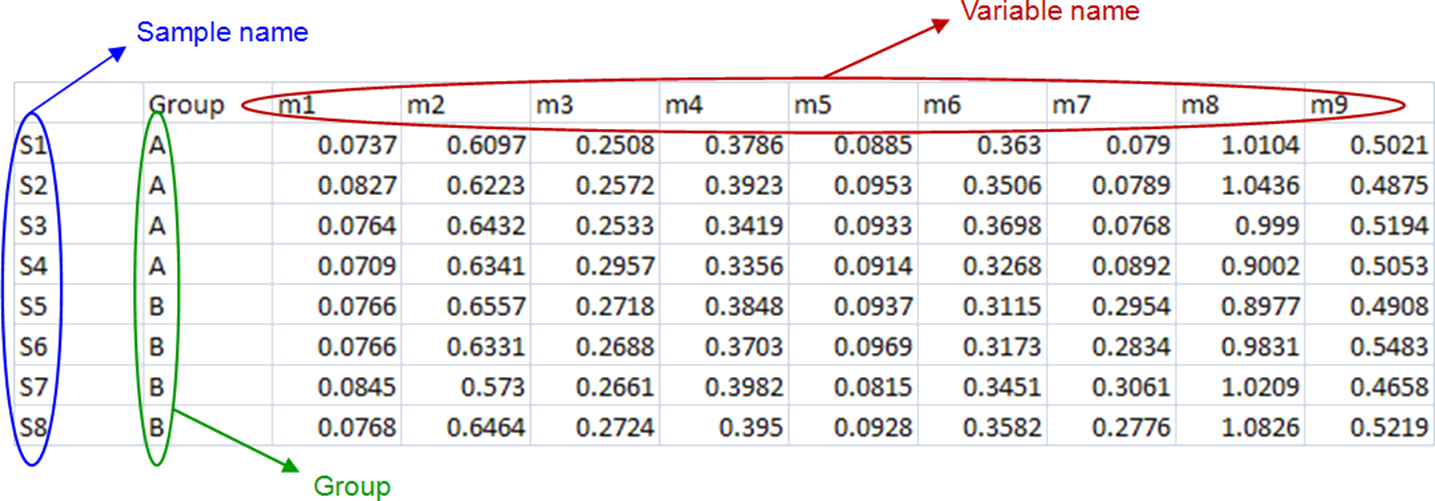
\includegraphics[width=0.85\textwidth]{images/input_spec.png} \\
    \caption[Input data format]{The standard format of the data matrix for statistical analyses.}
    \label{fig:input_spec}
\end{figure}


\section*{Currently available scripts}
\addcontentsline{toc}{section}{Currently available scripts}
Unless specified otherwise, the scripts in the ma-bioinformatics scripts repository use the input data format specified above. These scripts are still under development and generally have comments in them that describes what each step achieves.

These scripts are hosted at \url{http://code.google.com/p/ma-bioinformatics/} and can be downloaded from there as a zip package.
Examples provided below are created using the file \textsf{input.csv}, also provided in the download.

\newpage

\subsection*{General scripts}
\addcontentsline{toc}{subsection}{General scripts}

\subsubsection*{boxplot.r}
\addcontentsline{toc}{subsubsection}{boxplot.r}
This script will produce a boxplot for both samples (Figure \ref{fig:boxplot_smpl}) and variables (Figure \ref{fig:boxplot_var}). The top of the box is the 75th percentile (the median value of the upper half of the values, also called the upper quartile or Q$_3$) value and the bottom of the box is the 25th percentile (lower quartile, Q$_1$). The ends of the whiskers are the upper and lower values in the data set that are within 1.5 times the interquartile range (IQR), the difference between the first and third quartile, and any values outside of these are defined as outliers, represented by open circles.

\begin{figure}[!h]
    \centering
    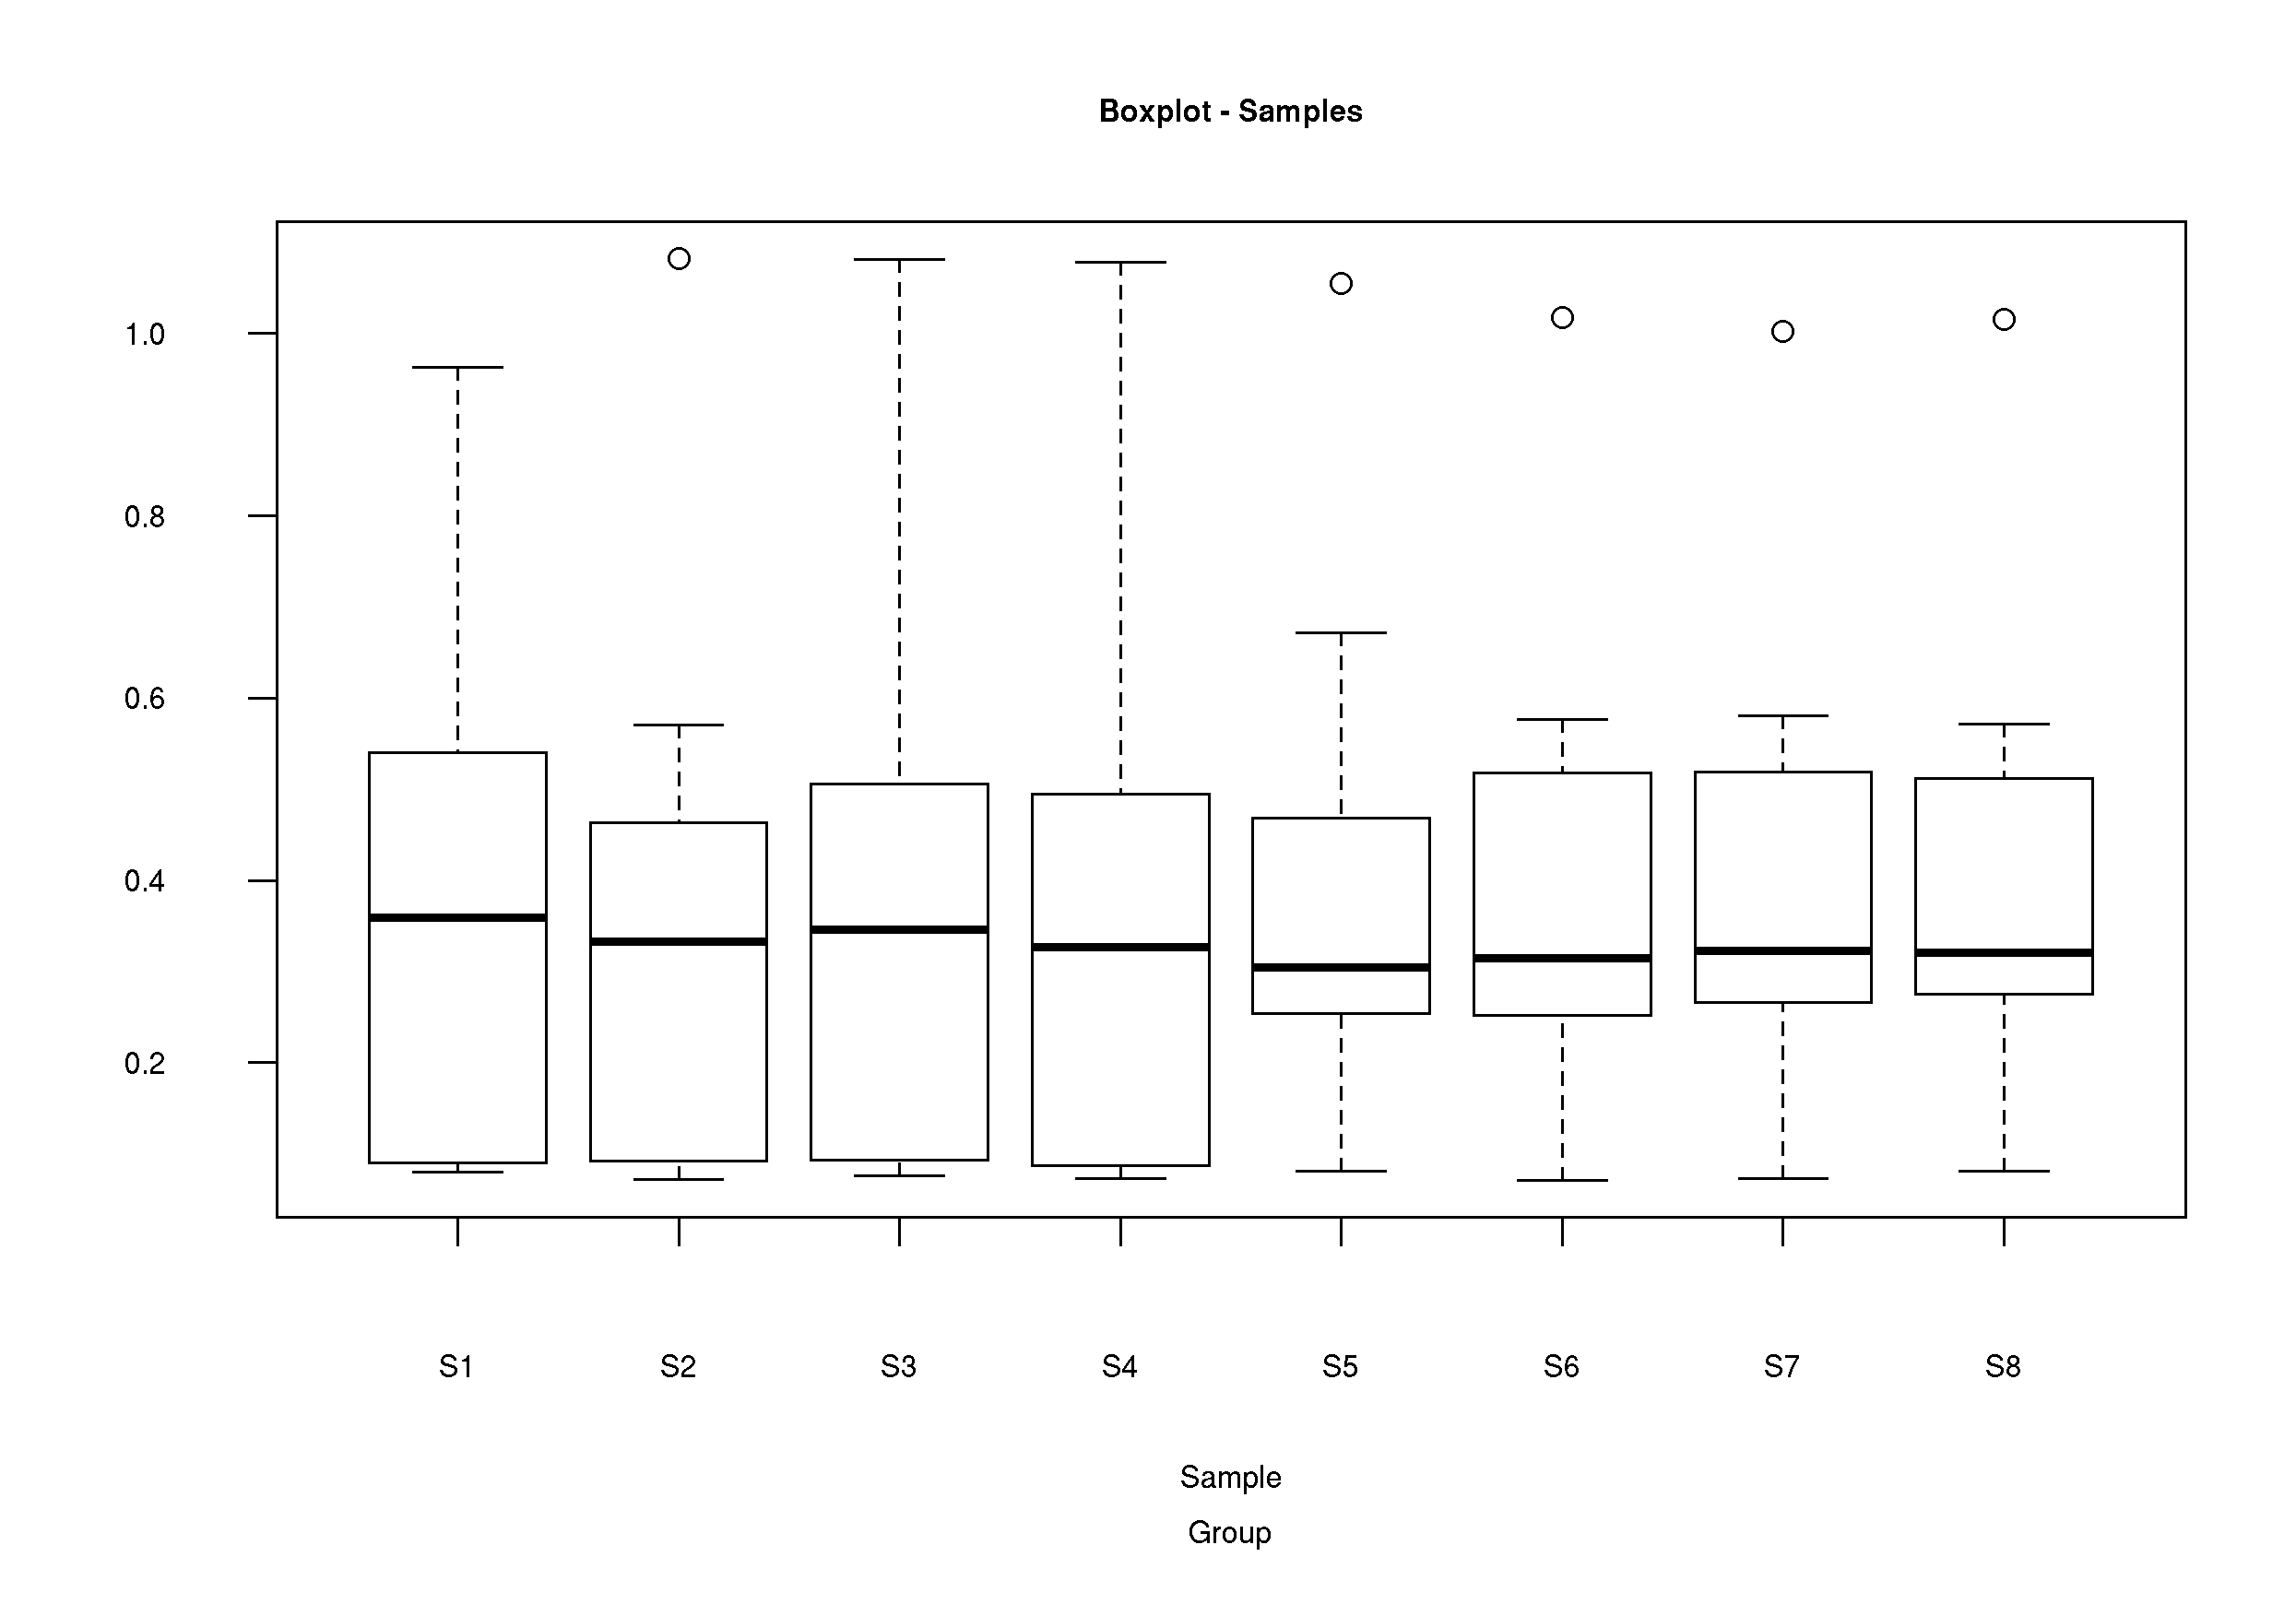
\includegraphics[width=0.85\textwidth]{images/boxplot_smpl.png} \\
    \caption[Boxplot - Samples]{Boxplot for samples using data from \textsf{input.csv}.}
    \label{fig:boxplot_smpl}
\end{figure}

\begin{figure}[!ht]
    \centering
    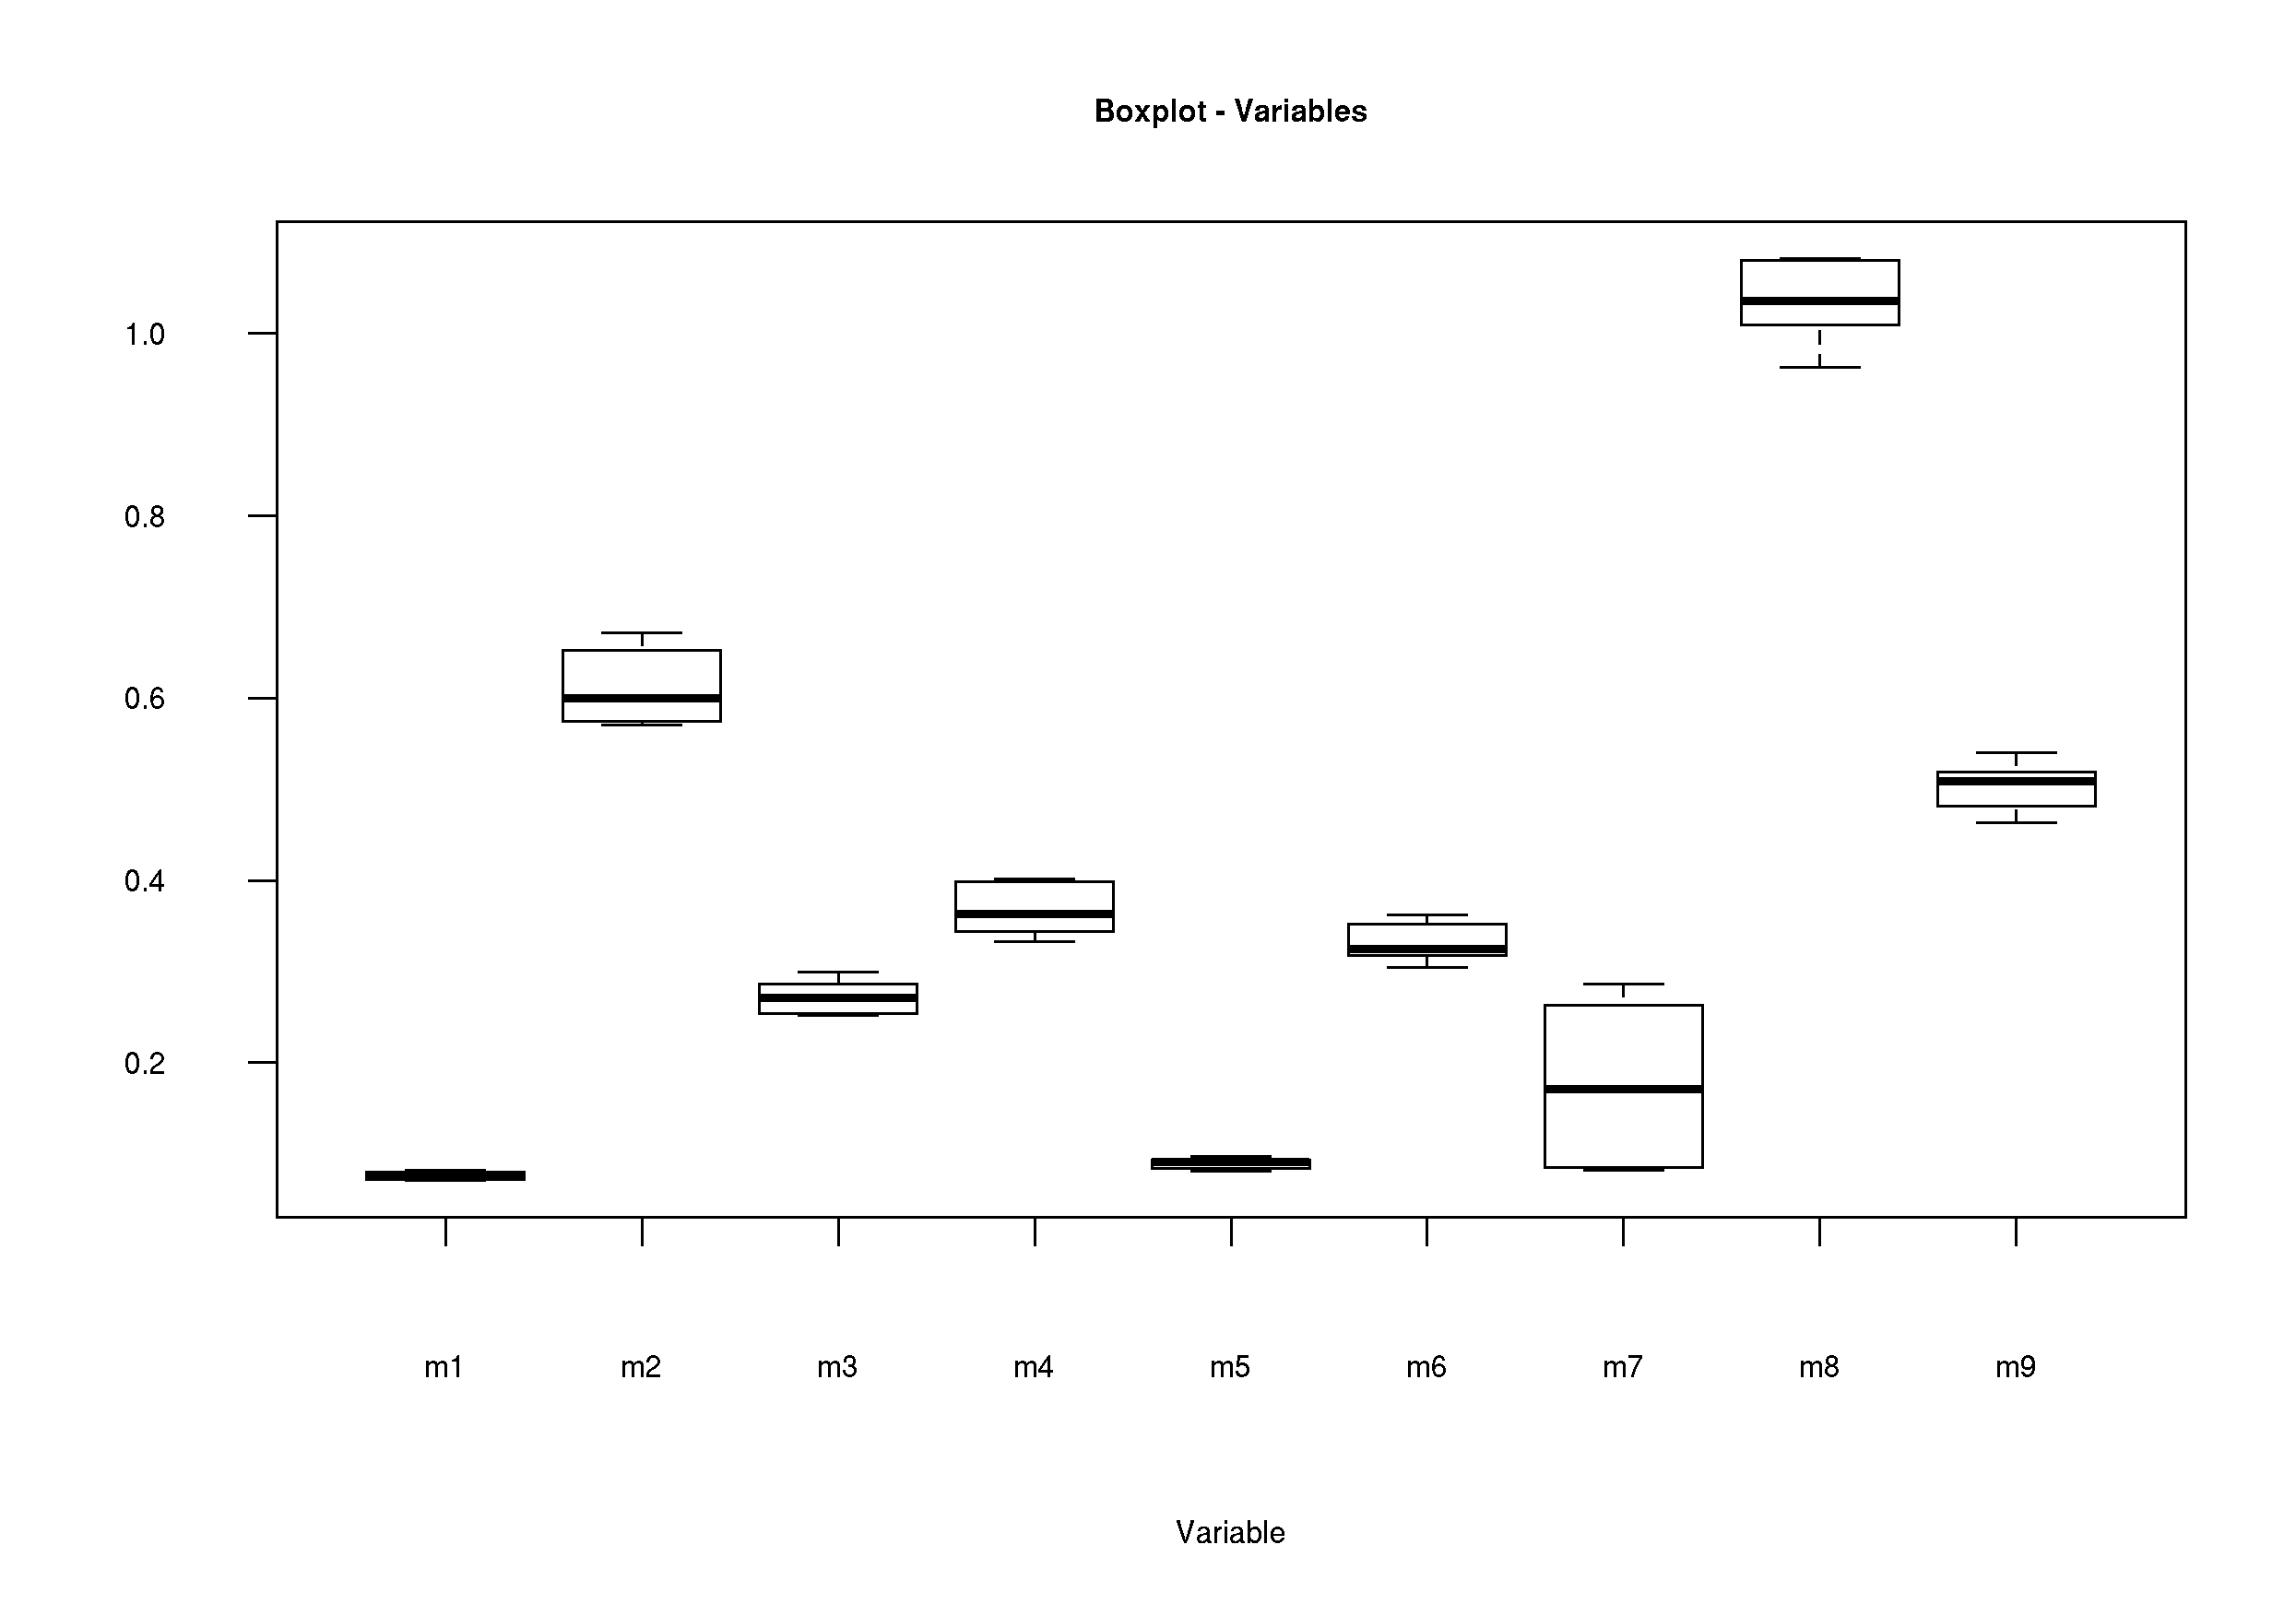
\includegraphics[width=0.85\textwidth]{images/boxplot_var.png} \\
    \caption[Boxplot - Variables]{Boxplot for variables using input.csv.}
    \label{fig:boxplot_var}
\end{figure}

\subsubsection*{mms\_plot.r}
\addcontentsline{toc}{subsubsection}{mms\_plot.r}
Produces a plot of the mean, median and standard deviation across all samples (Figure \ref{fig:MeanMedStdev_plot}). This enables a graphical overview of similarity of samples, and allows for rapid identification of outliers.
% This needs to be expanded - it's pretty minimal as it is, and if we expand the text we also have the added bonus of not having all the images in a big lump at the end!

\begin{figure}[!htb]
    \centering
    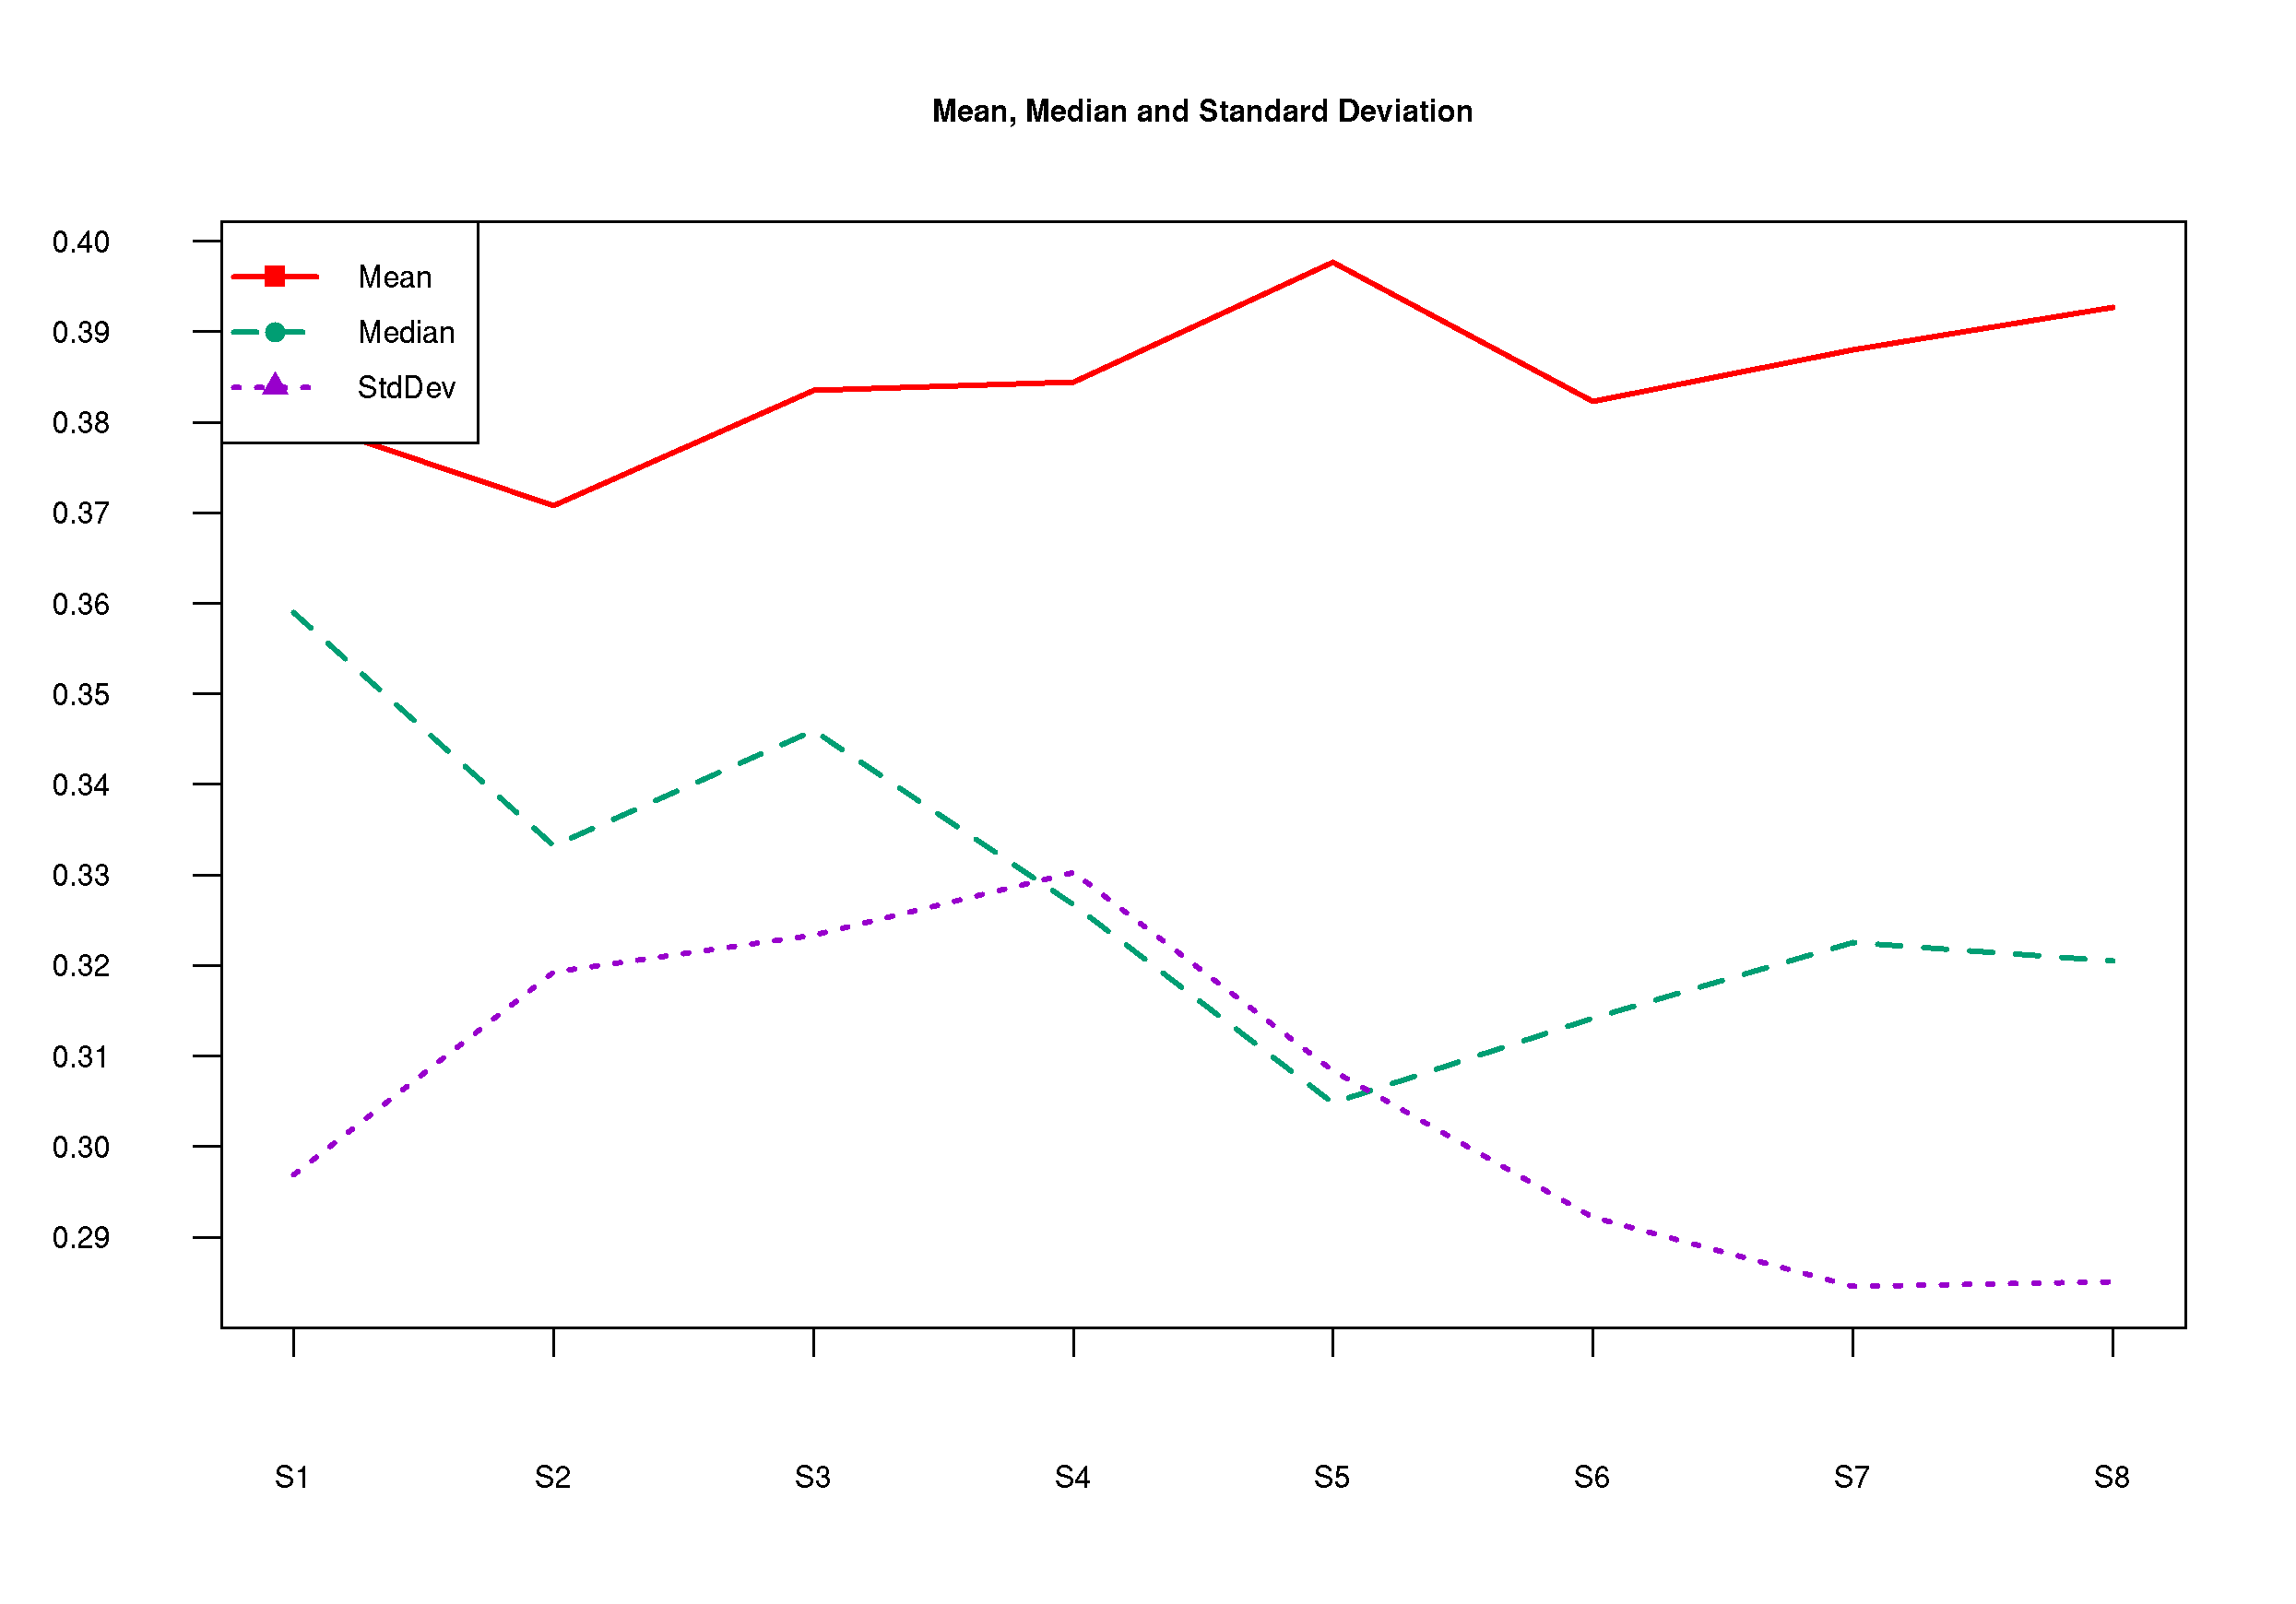
\includegraphics[width=0.85\textwidth]{images/MeanMedStdev_plot.png} \\
    \caption[Mean, Median and Standard Deviation]{Line plot showing the mean, median and standard deviation.}
    \label{fig:MeanMedStdev_plot}
\end{figure}

\subsubsection*{mean\_sd.r}
\addcontentsline{toc}{subsubsection}{mean\_sd.r}
It is important to explore a data set prior to choosing any normalisation or transformation method. Heteroscedastic noise (where the standard deviation of each metabolite in replicate samples changes with the mean of the metabolite) may change the results from the normalised data profoundly.

The optimal transformation to change heteroscedastic noise into homoscedastic noise depends on the structure of the heteroscedasticity in the signals. If the standard deviation is proportional to the mean of the signal (as in Figure \ref{fig:heterosced}), then a log transform is optimal to treat the data. If the standard deviation is proportional to the root of the mean then square root transformation provides a homoscedastic noise pattern (as in Figure \ref{fig:homosced}).

\begin{figure}[!hpt]
    \centering
    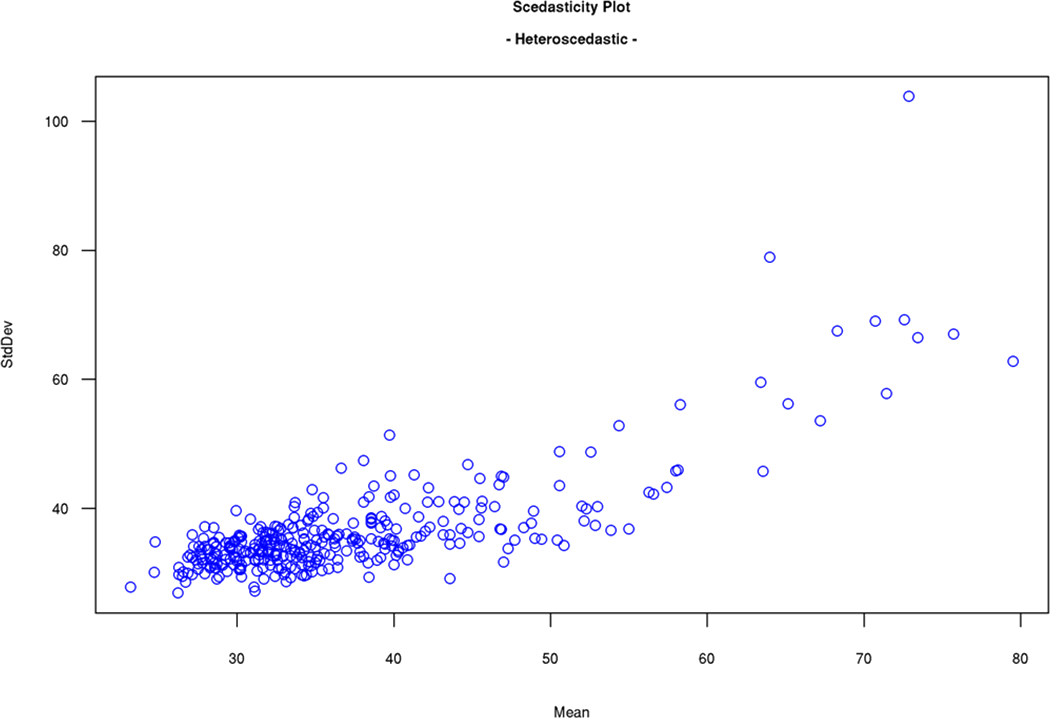
\includegraphics[width=0.85\textwidth]{images/heterosced.png} \\
    \caption[Heteroscedasticity]{Heteroscedastic data. The overall shape of the data is a fanned line, as the standard deviation increases with the size of the mean.}
    \label{fig:heterosced}
\end{figure}

\begin{figure}[!hpb]
    \centering
    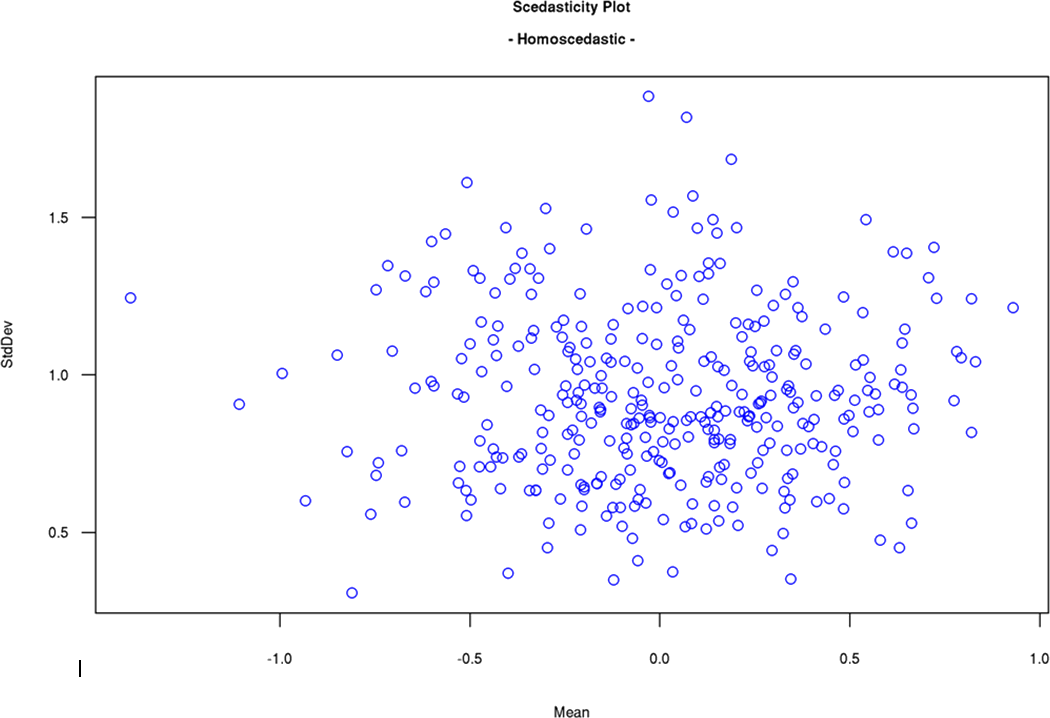
\includegraphics[width=0.85\textwidth]{images/homosced.png} \\
    \caption[Homoscedasticity]{Homoscedastic data. Points are distributed randomly over the plot, and standard deviation does not vary with the size of the mean.}
    \label{fig:homosced}
\end{figure}

\subsubsection*{t\_test.r}
\addcontentsline{toc}{subsubsection}{t\_test.r}
Performs a Student's \emph{t}-test, and outputs a .csv file with the p-values for each variable. This test assumes a normal distribution [\textsf{p\_t\_test.csv}].

\subsubsection*{m\_ttest.r}
\addcontentsline{toc}{subsubsection}{m\_ttest.r}
This function performs moderated one sample, two sample, and paired t tests, under the assumption of normally distributed data. The output is an excel file containing the metabolite names and corresponding moderated p-values.

\subsubsection*{wilcoxn.r}
\addcontentsline{toc}{subsubsection}{wilcoxn.r}
Performs Wilcoxon Rank Sum Test, a test that does not assume a normal distribution. Output is a .csv file containing the p-values for each varaible [\textsf{p\_wilcoxon\_test.csv}].

\subsubsection*{kruskal\_wallis.r}
\addcontentsline{toc}{subsubsection}{kruskal\_wallis.r}
This function performs a Kruskal-Wallis test,  a non-parametric test comparing three or more groups to identify which are significantly different. The output is a .csv file containing the metabolite names and corresponding moderated p-values [\textsf{kw\_pvals.csv}]. The script also allows for the identification of which groups are significantly different for a selected metabolite. In this case, a second file, \textsf{kwMultComp\_\{metabolite name\}.csv} will also be produced.

\subsubsection*{fold\_chg.r}
\addcontentsline{toc}{subsubsection}{fold\_chg.r}
Calculates the fold change from the (alphanumerically) first group in the data matrix (i.e. for our example input data, this would be fold change from group A). Fold change is calculated by determining the mean for each variable in each sample, and then dividing each mean by the mean for the first group. If the value is less than 1, the returned value is the negative inverse (i.e. if
$\frac{mean_{expt}}{mean_{ctrl}} > 1$, no change; if $\frac{mean_{expt}}{mean_{ctrl}} < 1 $, then fold change $= -1\times\frac{mean_{ctrl}}{mean_{expt}}$. It returns a table of the means as well as the table of fold changes.

\subsubsection*{volcano\_plot.r}
\addcontentsline{toc}{subsubsection}{volcano\_plot.r}
A volcano plot is a type of scatter plot which shows fold change on the \emph{x}-axis and the statistical significance (p-values from a \emph{t}-test) on the \emph{y}-axis. It readily shows which metabolites have large magnitude changes that are statistically significant between two conditions.

\begin{figure}[!htb]
    \centering
    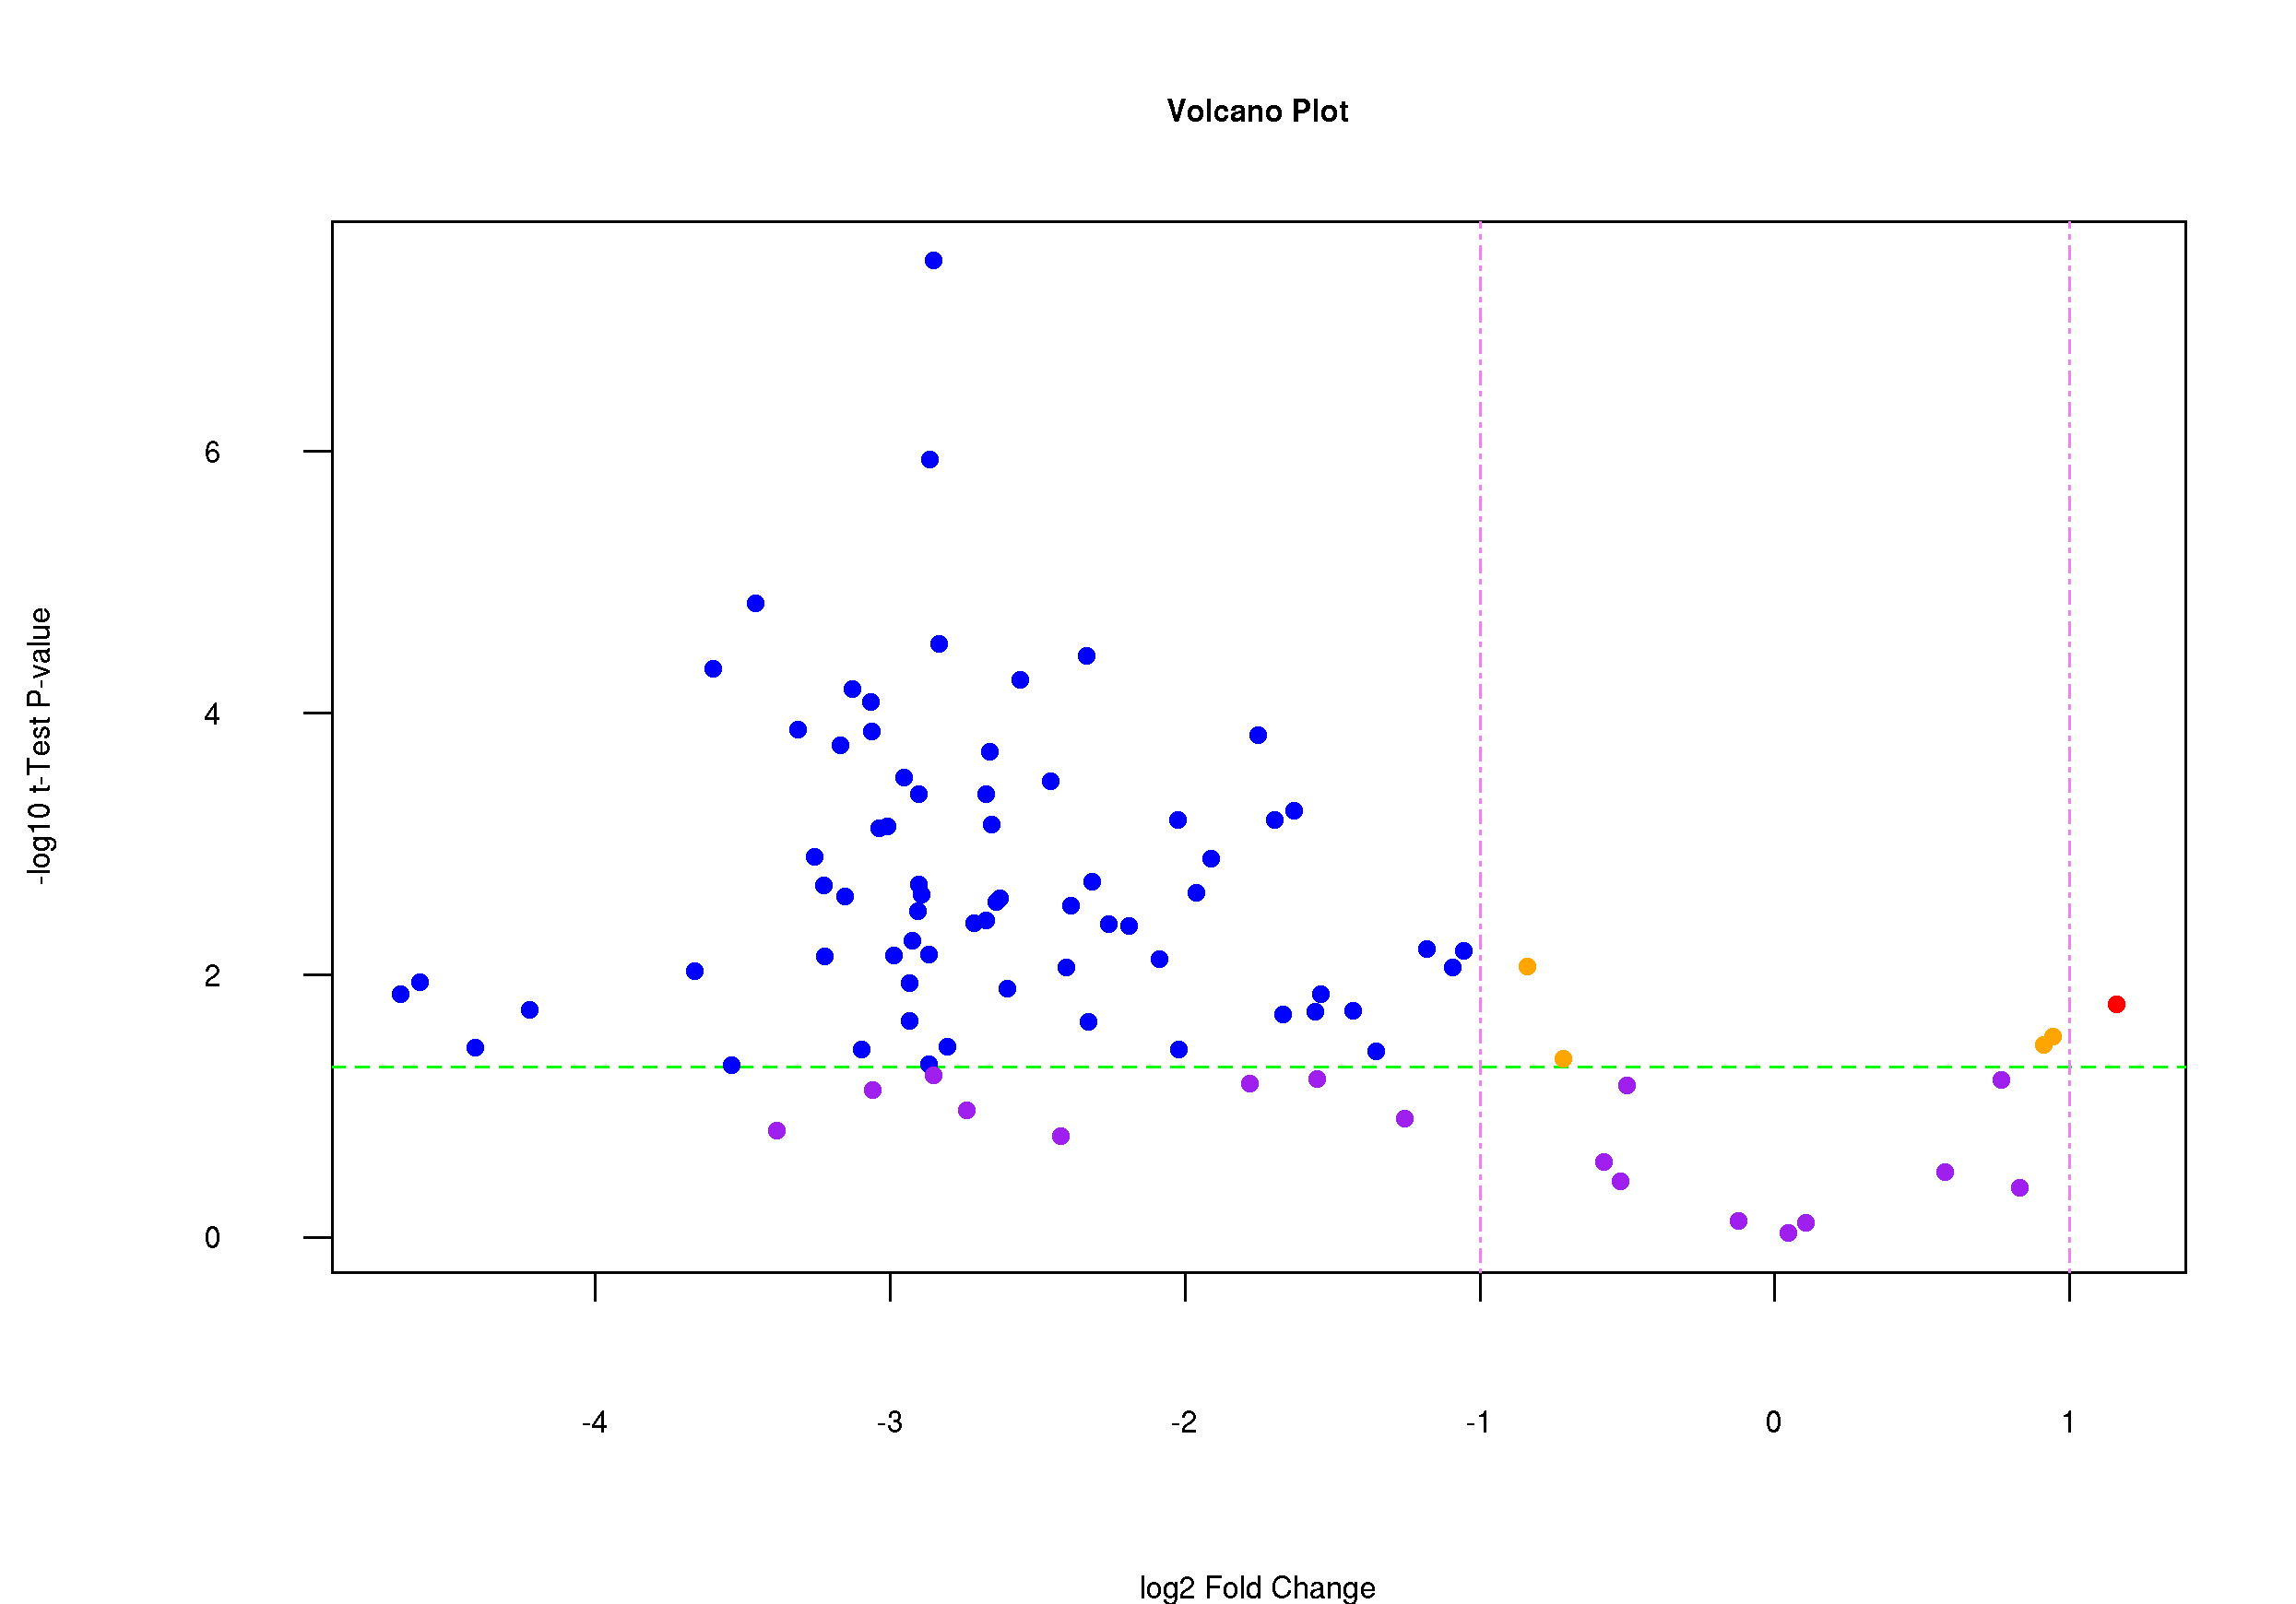
\includegraphics[width=0.85\textwidth]{images/volcano_plot.png} \\
    \caption[Volcano plot]{Volcano plot.}
    \label{fig:volcano_plot}
\end{figure}

\subsubsection*{correlation.r}
\addcontentsline{toc}{subsubsection}{correlation.r}
This script calculates the correlation between the variables (metabolites) in a data set. The output [\textsf{cor\_matrix.csv}] is a correlation matrix that can be used to draw a heat map (using the \textsf{heatmap.r} script, the output of which is shown in figure \ref{fig:cor_heatmap}), an example of which is presented in table \ref{tab:cor_mat}. The output \textsf{cor\_variables.csv} gives a .csv file in which the correlation coefficients  between all the variables  are ordered in decreasing values of correlation co-efficient (table \ref{tab:cor_var}).

\begin{table}[!h]
    \caption[Correlation matrix]{Output correlation matrix.}
    \begin{center}
        \begin{tabular}{lrrrrrrrrr}
        \toprule
          & m1 & m2 & m3 & m4 & m5 & m6 & m7 & m8 & m9\\
        \midrule
          m1 & 1 & -0.551 & -0.407 & 0.696 & -0.319 & 0.142 & 0.344 & 0.512 & -0.527\\
          m2 & -0.551 & 1 & 0.234 & -0.358 & 0.821 & -0.236 & -0.052 & -0.308 & 0.580\\
          m3 & -0.407 & 0.234 & 1 & -0.326 & 0.042 & -0.619 & 0.230 & -0.546 & 0.066\\
          m4 & 0.696 & -0.358 & -0.326 & 1 & -0.260 & 0.033 & 0.553 & 0.546 & -0.407\\
          m5 & -0.319 & 0.821 & 0.042 & -0.260 & 1 & -0.259 & -0.155 & -0.121 & 0.690\\
          m6 & 0.142 & -0.236 & -0.619 & 0.033 & -0.259 & 1 & -0.502 & 0.714 & -0.078\\
          m7 & 0.344 & -0.052 & 0.230 & 0.553 & -0.155 & -0.502 & 1 & 0.024 & 0.004\\
          m8 & 0.512 & -0.308 & -0.546 & 0.546 & -0.121 & 0.714 & 0.024 & 1 & 0.041\\
          m9 & -0.527 & 0.580 & 0.066 & -0.407 & 0.690 & -0.078 & 0.004 & 0.041 & 1\\
        \bottomrule
        \end{tabular}
    \end{center}
    \label{tab:cor_mat}
\end{table}

\begin{figure}[!h]
    \centering
    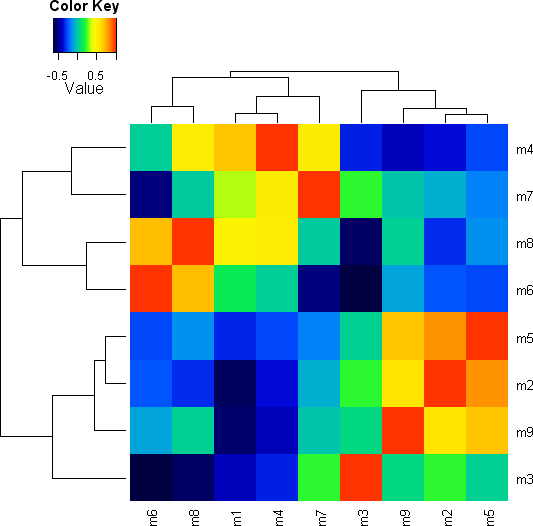
\includegraphics[width=0.85\textwidth]{images/cor_heatmap.png} \\
    \caption[Correlation heatmap]{Heatmap of the correlation matrix (drawn using \textsf{heatmap.r} script)}
    \label{fig:cor_heatmap}
\end{figure}

\begin{table}[!h]
\caption[Correlation between variables]{Output \textsf{cor\_variables.csv} file}
    \begin{center}
        \begin{tabular}{ccc}
        \toprule
          Variable\_1 & Variable\_2 & cor\_coefficient\\
        \midrule
          m5 & m2 & 0.821\\
          m8 & m6 & 0.714\\
          m4 & m1 & 0.696\\
          m9 & m5 & 0.690\\
          m9 & m2 & 0.580\\
          m7 & m4 & 0.553\\
          m8 & m4 & 0.546\\
          m8 & m1 & 0.512\\
          m7 & m1 & 0.344\\
          m3 & m2 & 0.234\\
          m7 & m3 & 0.230\\
          m6 & m1 & 0.142\\
          m9 & m3 & 0.066\\
          m5 & m3 & 0.042\\
          m9 & m8 & 0.041\\
          m6 & m4 & 0.033\\
          m8 & m7 & 0.024\\
          m9 & m7 & 0.004\\
          m7 & m2 & -0.052\\
          m9 & m6 & -0.078\\
          m8 & m5 & -0.121\\
          m7 & m5 & -0.155\\
          m6 & m2 & -0.236\\
          m6 & m5 & -0.259\\
          m5 & m4 & -0.260\\
          m8 & m2 & -0.308\\
          m5 & m1 & -0.319\\
          m4 & m3 & -0.326\\
          m4 & m2 & -0.358\\
          m3 & m1 & -0.407\\
          m9 & m4 & -0.407\\
          m7 & m6 & -0.502\\
          m9 & m1 & -0.527\\
          m8 & m3 & -0.546\\
          m2 & m1 & -0.551\\
          m6 & m3 & -0.619\\
        \bottomrule
        \end{tabular}
    \end{center}
\label{tab:cor_var}
\end{table}

\subsubsection*{z-score.r}
\addcontentsline{toc}{subsubsection}{z-score.r}
This function assumes that the input data has been normalised and transformed appropriately. If that is the case, then running this script will produce a plot of variables against the z-score for each of the variable. The z-score is calculated as $z=\frac{x-\mu}{\sigma}$, where x is the value of the variable to be normalised, $\mu$ is the mean and $\sigma$ is the standard deviation of the variable for that group.

\subsection*{Transformation}
\addcontentsline{toc}{subsection}{Transformation}
This is an operation that is applied to each variable, and the type of transformation applied depends on the statistical test that is necessary to answer a biological question. For example, a t-test assumes that the data is normally distributed, hence it is important to transform a right- or left-skewed data set to a normal distribution.

\subsubsection*{log.r}
\addcontentsline{toc}{subsubsection}{log.r}
Performs a log$_{10}$ transform of the input data, and generates a new data matrix [\textsf{log\_transform.csv}].

\subsection*{Normalisation}
\addcontentsline{toc}{subsection}{Normalisation}
This process is applied to the entire data set, and enables samples to be directly compared to one another by reducing the influence that is non-biological in origin. As an example, running samples on different days can cause samples to appear different when in actual fact they are the same. Normalisation attempt to removes this influence so that samples from different groups can directly be compared. The output of these scripts are all .csv files.

\subsubsection*{norm\_is.r}
\addcontentsline{toc}{subsubsection}{norm\_is.r}
Uses an internal standard (in the column immediately following the ``Group'' column) to normalise the data set [\textsf{norm\_data\_IS.csv}].

\subsubsection*{norm\_ext\_vec.r}
\addcontentsline{toc}{subsubsection}{norm\_ext\_vec.r}
Uses an external vector (e.g. creatinine for urine samples saved as a separate file) to normalise the data set [\textsf{norm\_data\_ext\_vec.csv}].

\subsubsection*{norm\_median.r}
\addcontentsline{toc}{subsubsection}{norm\_median.r}
Takes the median value for each sample (i.e. row) and uses this value to normalise the data set [\textsf{norm\_data\_median.csv}].

\subsubsection*{norm\_Zscore.r}
\addcontentsline{toc}{subsubsection}{norm\_Zscore.r}
\emph{Z} score is a measure of how many standard deviations a sample is from the mean. This script calculates the \emph{Z} score for each sample and uses that value to normalise the data set [\textsf{norm\_data\_zscore.csv}].

\subsubsection*{norm\_sum.r}
\addcontentsline{toc}{subsubsection}{norm\_sum.r}
This script normalises the values on a per-sample basis by taking the sum of all values for each sample and using that value as the normalisation factor [\textsf{norm\_data\_sum.csv}].

\subsubsection*{norm\_quantile.r}
\addcontentsline{toc}{subsubsection}{norm\_quantile.r}
This script normalises the data based upon quantiles of each sample [\textsf{norm\_data\_quantile.csv}].

\subsection*{Cluster analysis}
\addcontentsline{toc}{subsection}{Cluster analysis}

\subsubsection*{hca.r}
\addcontentsline{toc}{subsubsection}{hca.r}
Hierarchical cluster analysis (HCA) is a technique that identifies groups of samples that show similar characteristics, and then quantifies the structural characteristics of the sample (or variable) data by constructing a hierarchy in a tree-like structure. There are two kinds of procedures that are commonly used to construct the tree, namely agglomerative and divisive. In an agglomerative procedure, each sample (or variable) starts in a cluster of its won, and then continually joins clusters until there is only one cluster containing all samples. The divisive method operates in the exact reverse.

This script uses complete linkage method but other different linkage measures can be used in HCA, including average, single and Ward's, which may result in different clusters.  The main objective of HCA is to classify the data into groups by structuring it, which helps to identify relationships among observations (samples/variables).

This script uses Manhattan distance to calculate the similarity, but other methods can be used by changing \textsf{``manhattan''} to one of \textsf{``euclidean''}, \textsf{``maximum''}, \textsf{``canberra''}, \textsf{``binary''} or \textsf{``minkowski''}.

It will generate a plot of both the sample distances (see Figure \ref{fig:HCA_smpl}) as well as the distance for the variables (Figure \ref{fig:HCA_var}).

\begin{figure}[!h!tb]
    \centering
    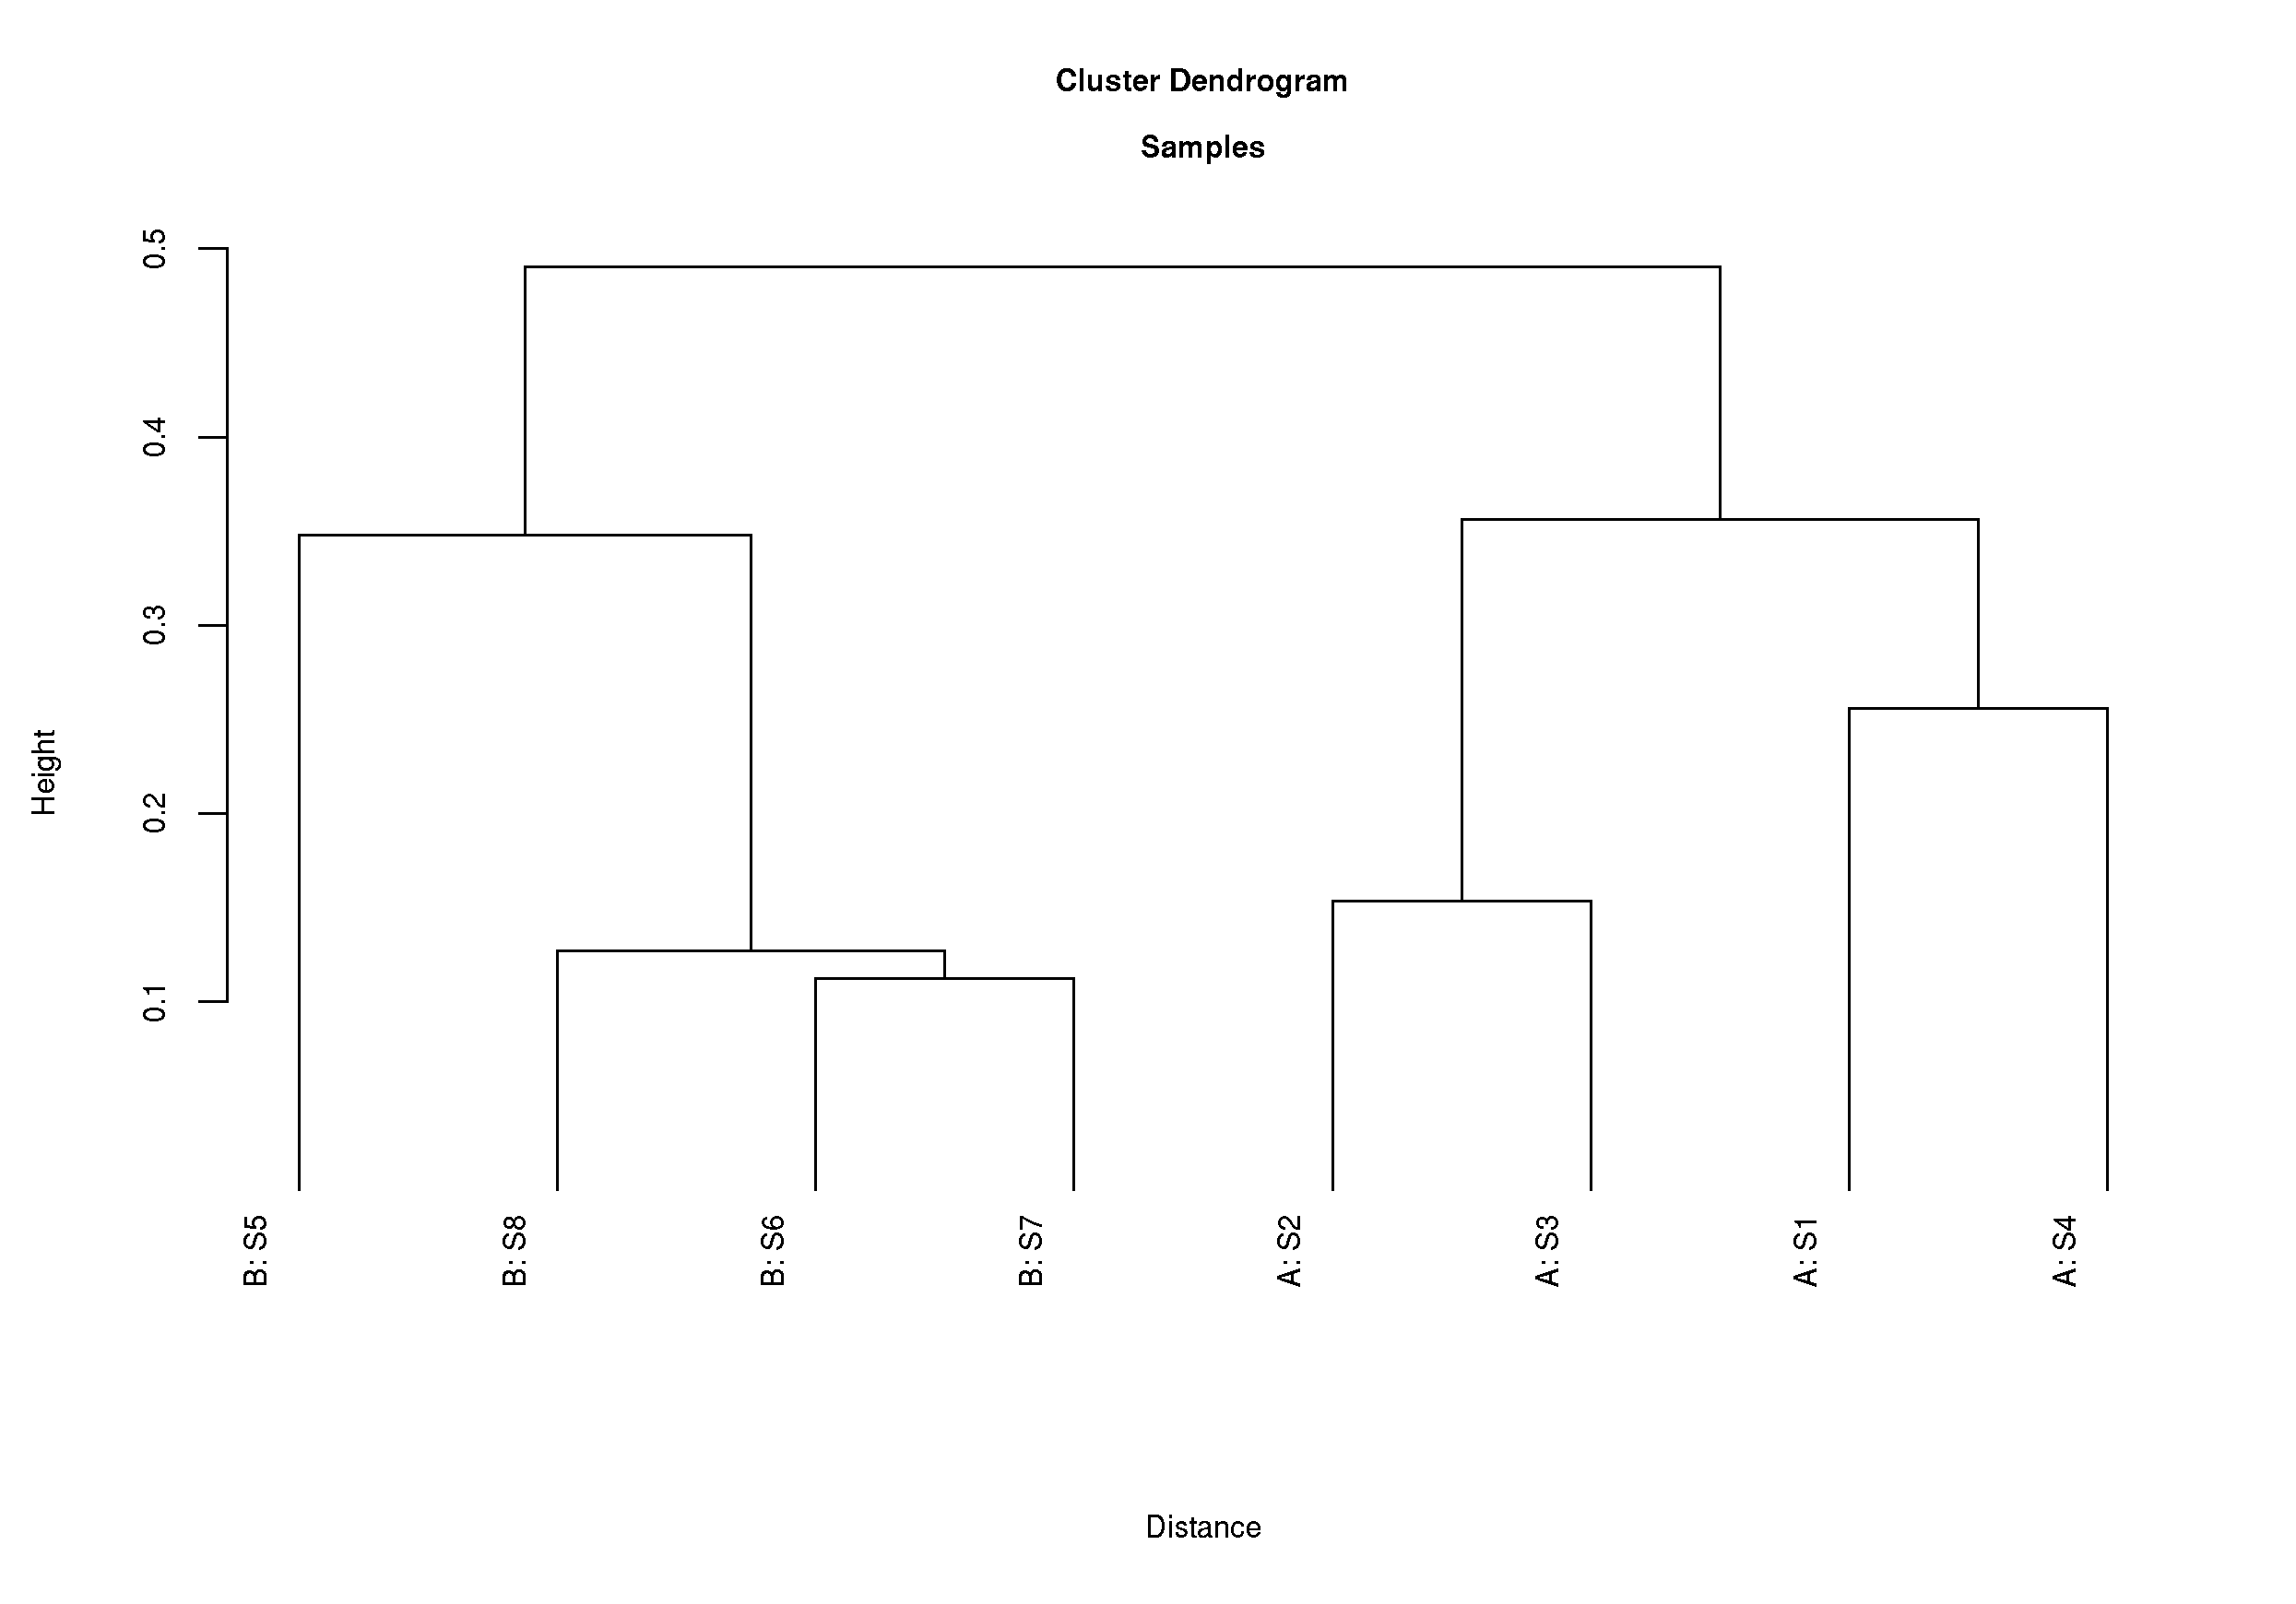
\includegraphics[width=0.85\textwidth]{images/HCA_smpl.png} \\
    \caption[HCA - Samples]{Hierarchical Cluster Analysis (HCA) for samples. Group labels are incorporated in the names on the leaves of the dendogram.}
    \label{fig:HCA_smpl}
\end{figure}

\begin{figure}[!ht!b]
    \centering
    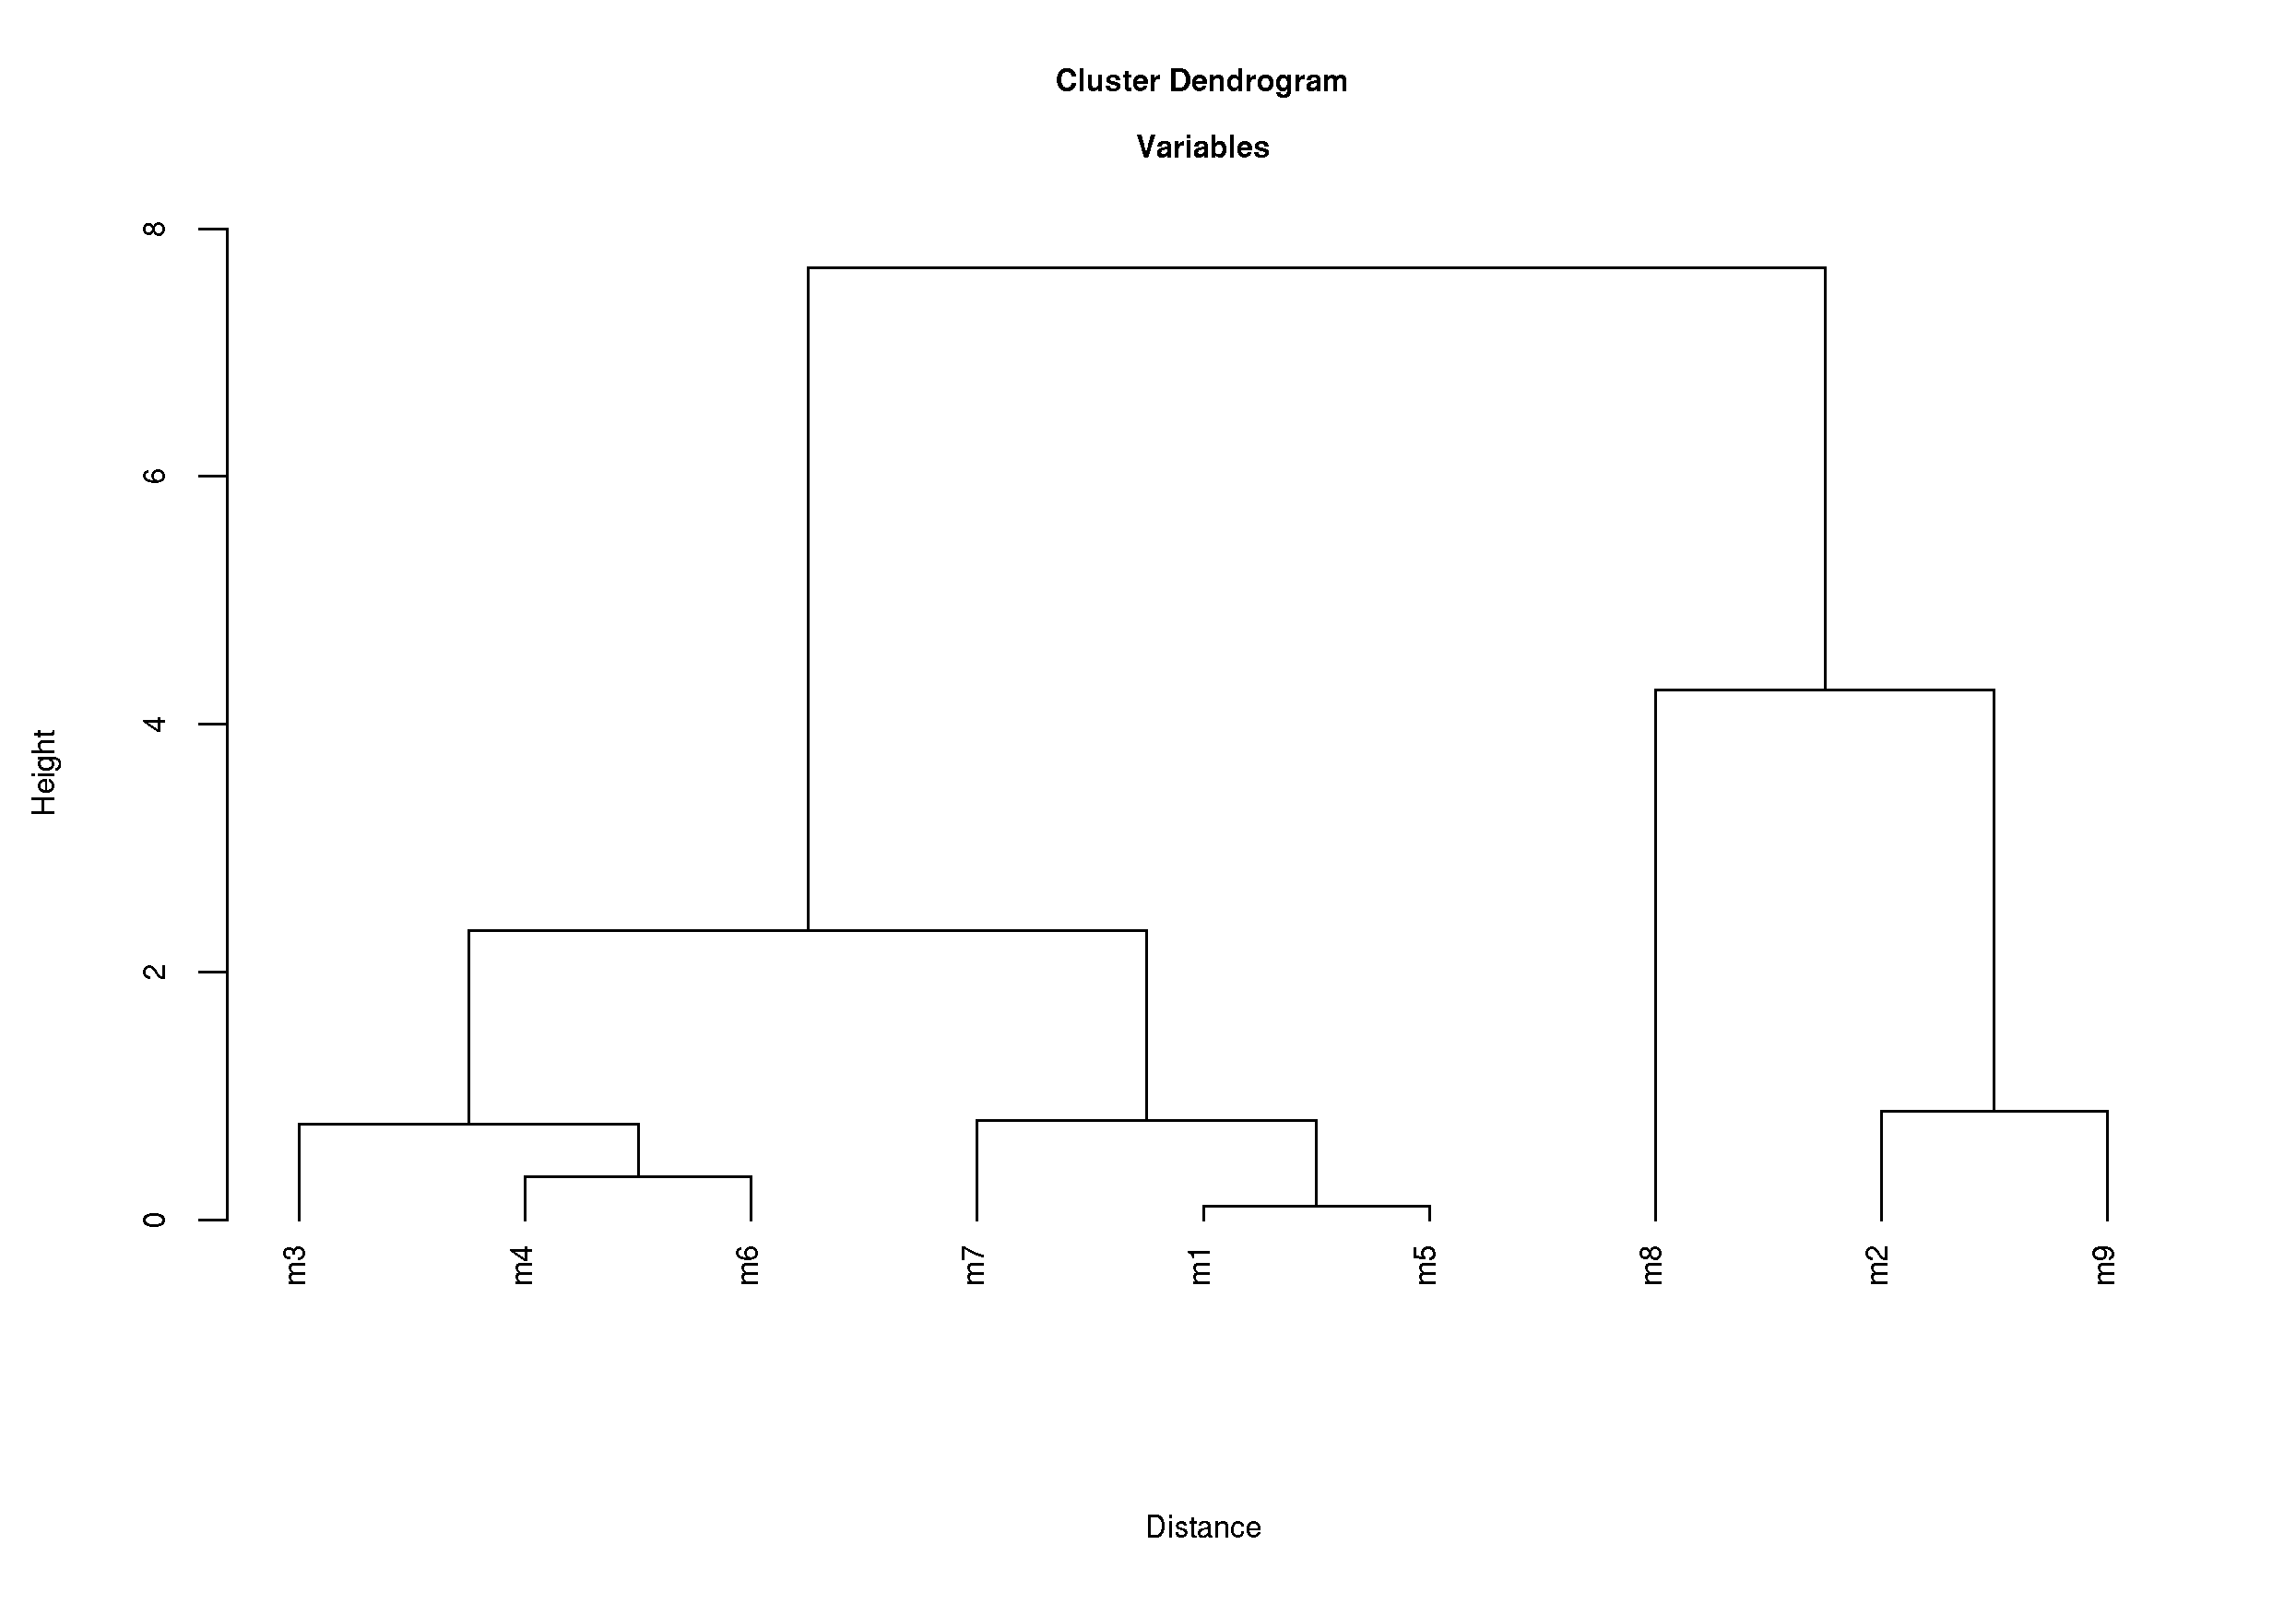
\includegraphics[width=0.85\textwidth]{images/HCA_var.png} \\
    \caption[HCA - Variables]{HCA for variables.}
    \label{fig:HCA_var}
\end{figure}

\subsubsection*{pca.r}
\addcontentsline{toc}{subsubsection}{pca.r}
Principal Component Analysis (PCA) is a data transformation technique which is used to reduce a multidimensional data set to a lower number of dimensions for further analysis. In PCA, a data set of interrelated variables is transformed to a new set of variables called principal components (PCs) in such a way that they are uncorrelated, and the first few of these PCs retain most of the variation present in the entire data set. The first PC is a linear combination of all the actual variables in such a way that it has the greatest amount of variation, and the second PC is a combination of the variables that have the next greatest variation in the remaining PCs.

This script produces multiple plots -- residual variance (Figure \ref{fig:PCA_variance}), scores plot labelled with sample names (Figure \ref{fig:PCA_scores_smpl}), scores plot labelled with group names (Figure \ref{fig:PCA_scores_grp}) and a loading plot (Figure \ref{fig:PCA_loadings}).

\begin{figure}[!hp]
    \centering
    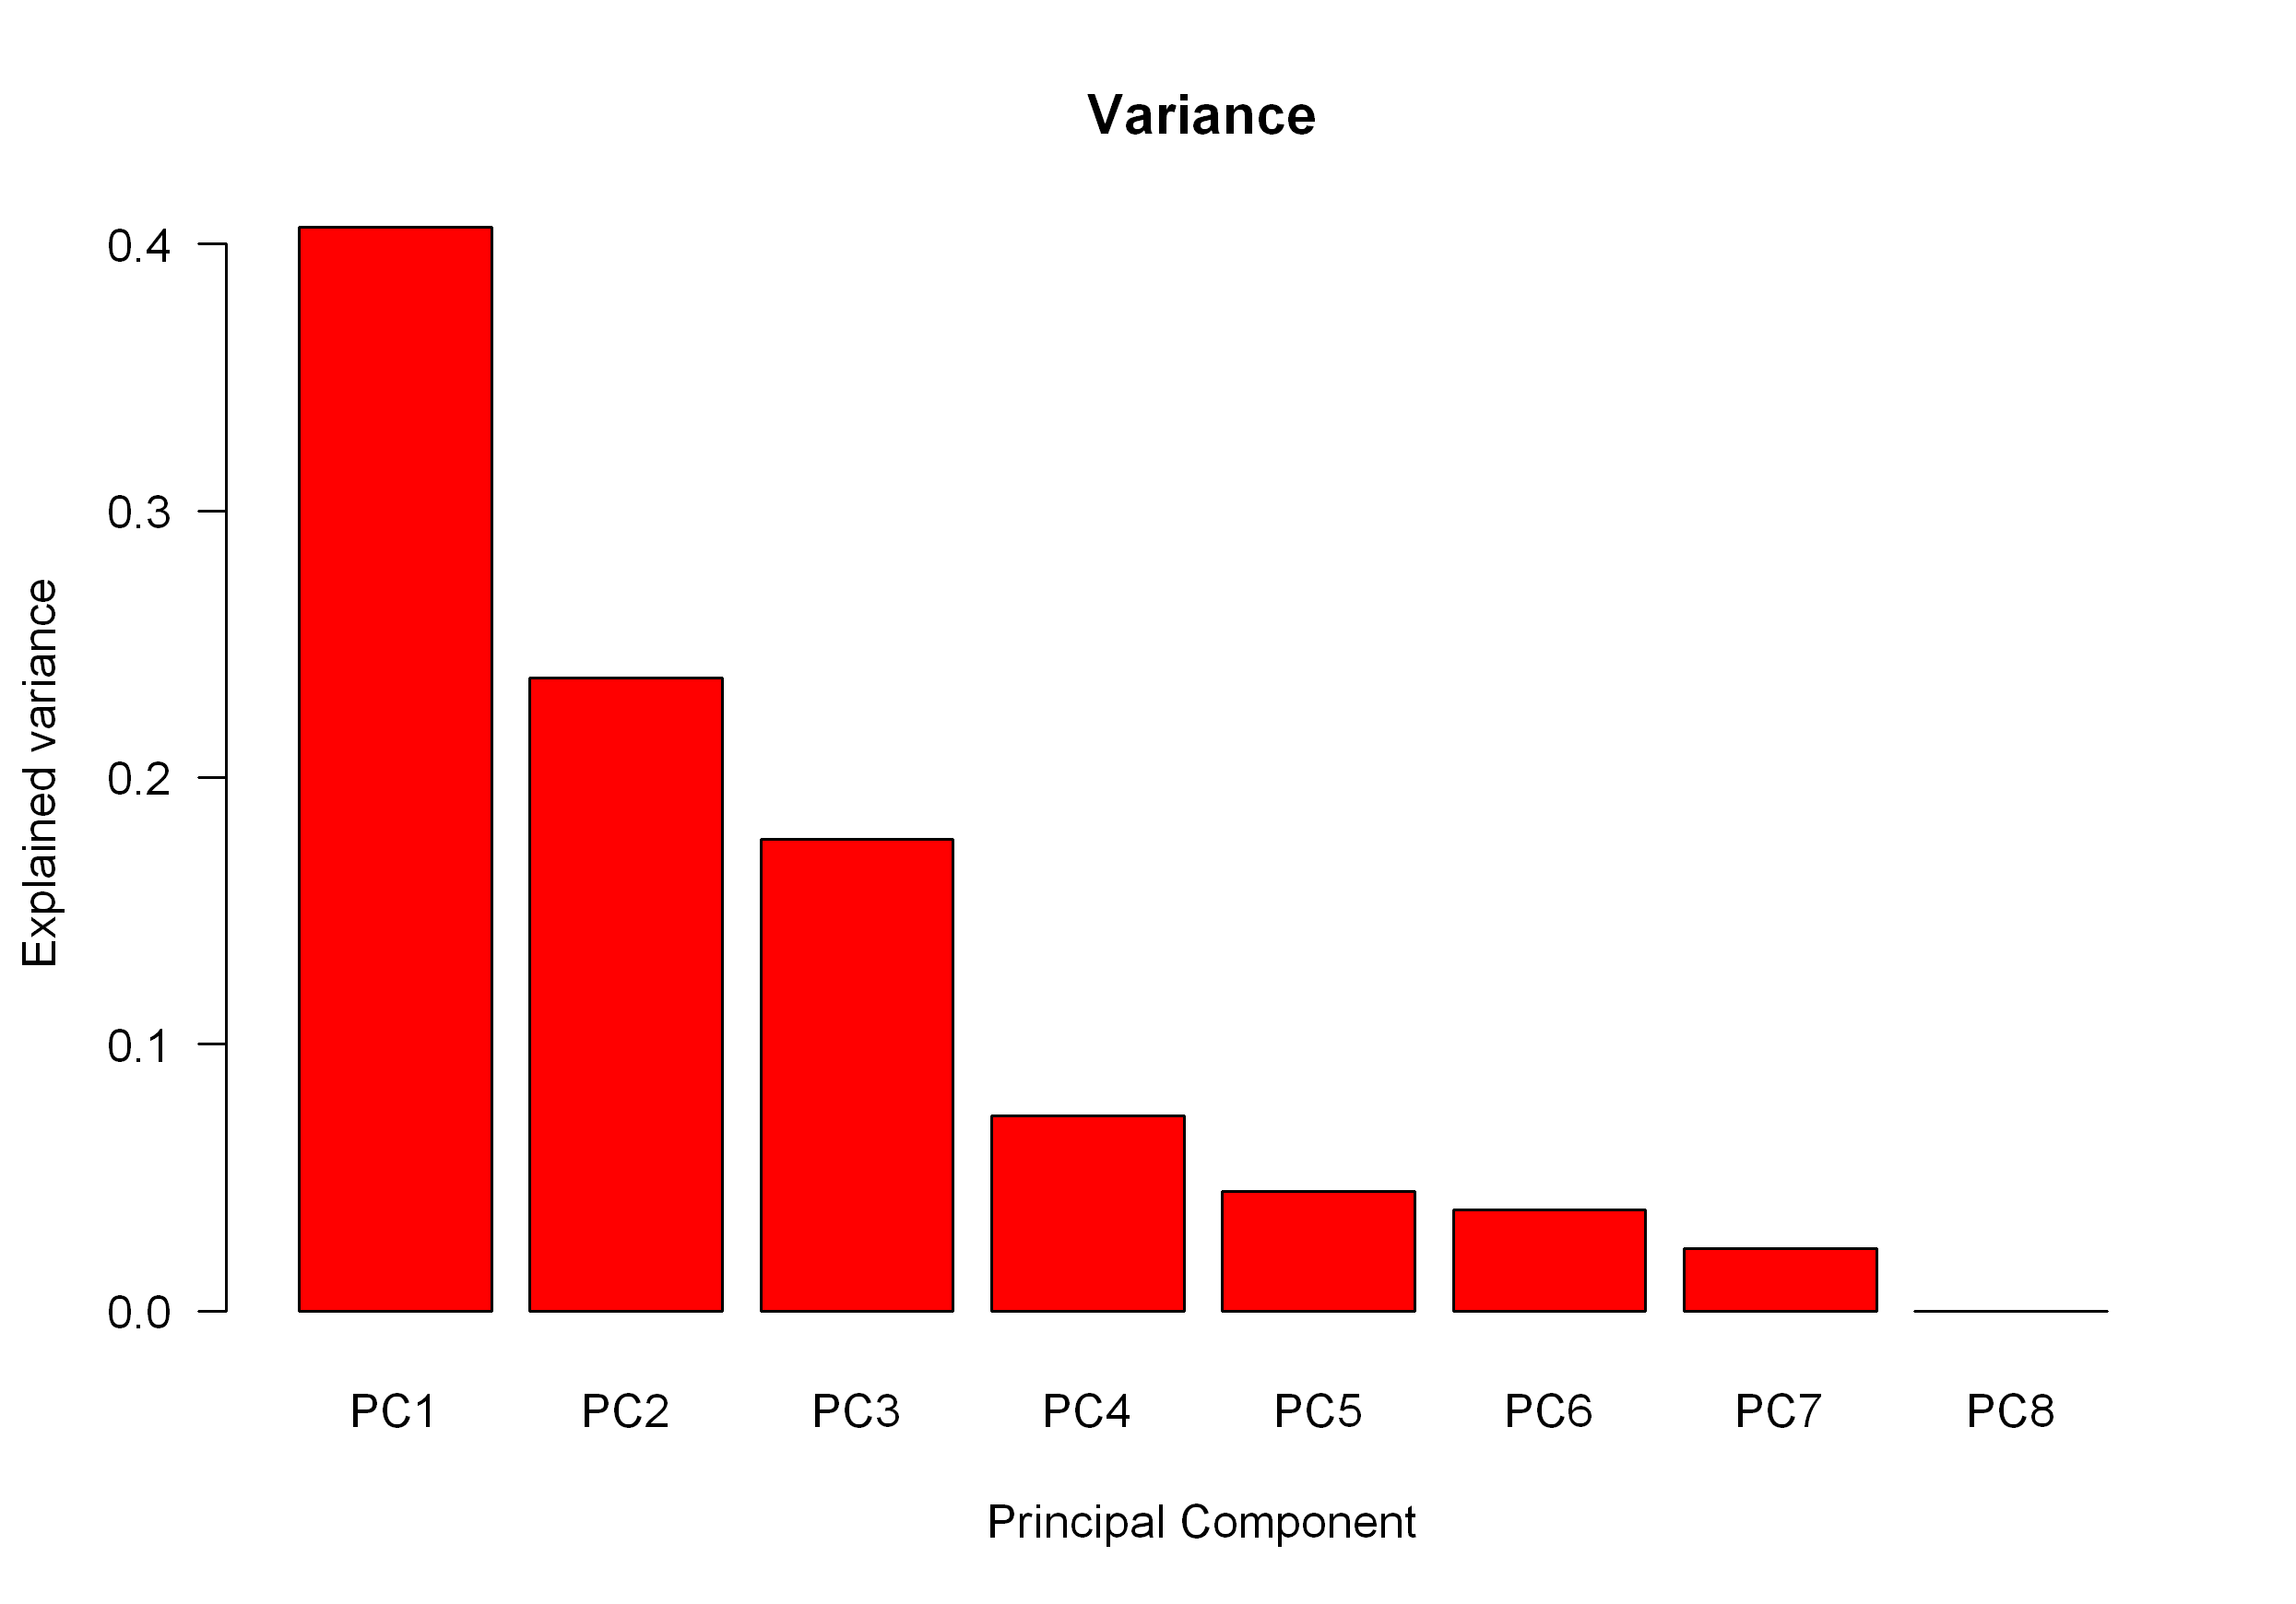
\includegraphics[width=0.85\textwidth]{images/PCA_variance.png} \\
    \caption[PCA - Variance]{Residual variance plot.}
    \label{fig:PCA_variance}
\end{figure}

\begin{figure}[!h!tp]
    \centering
    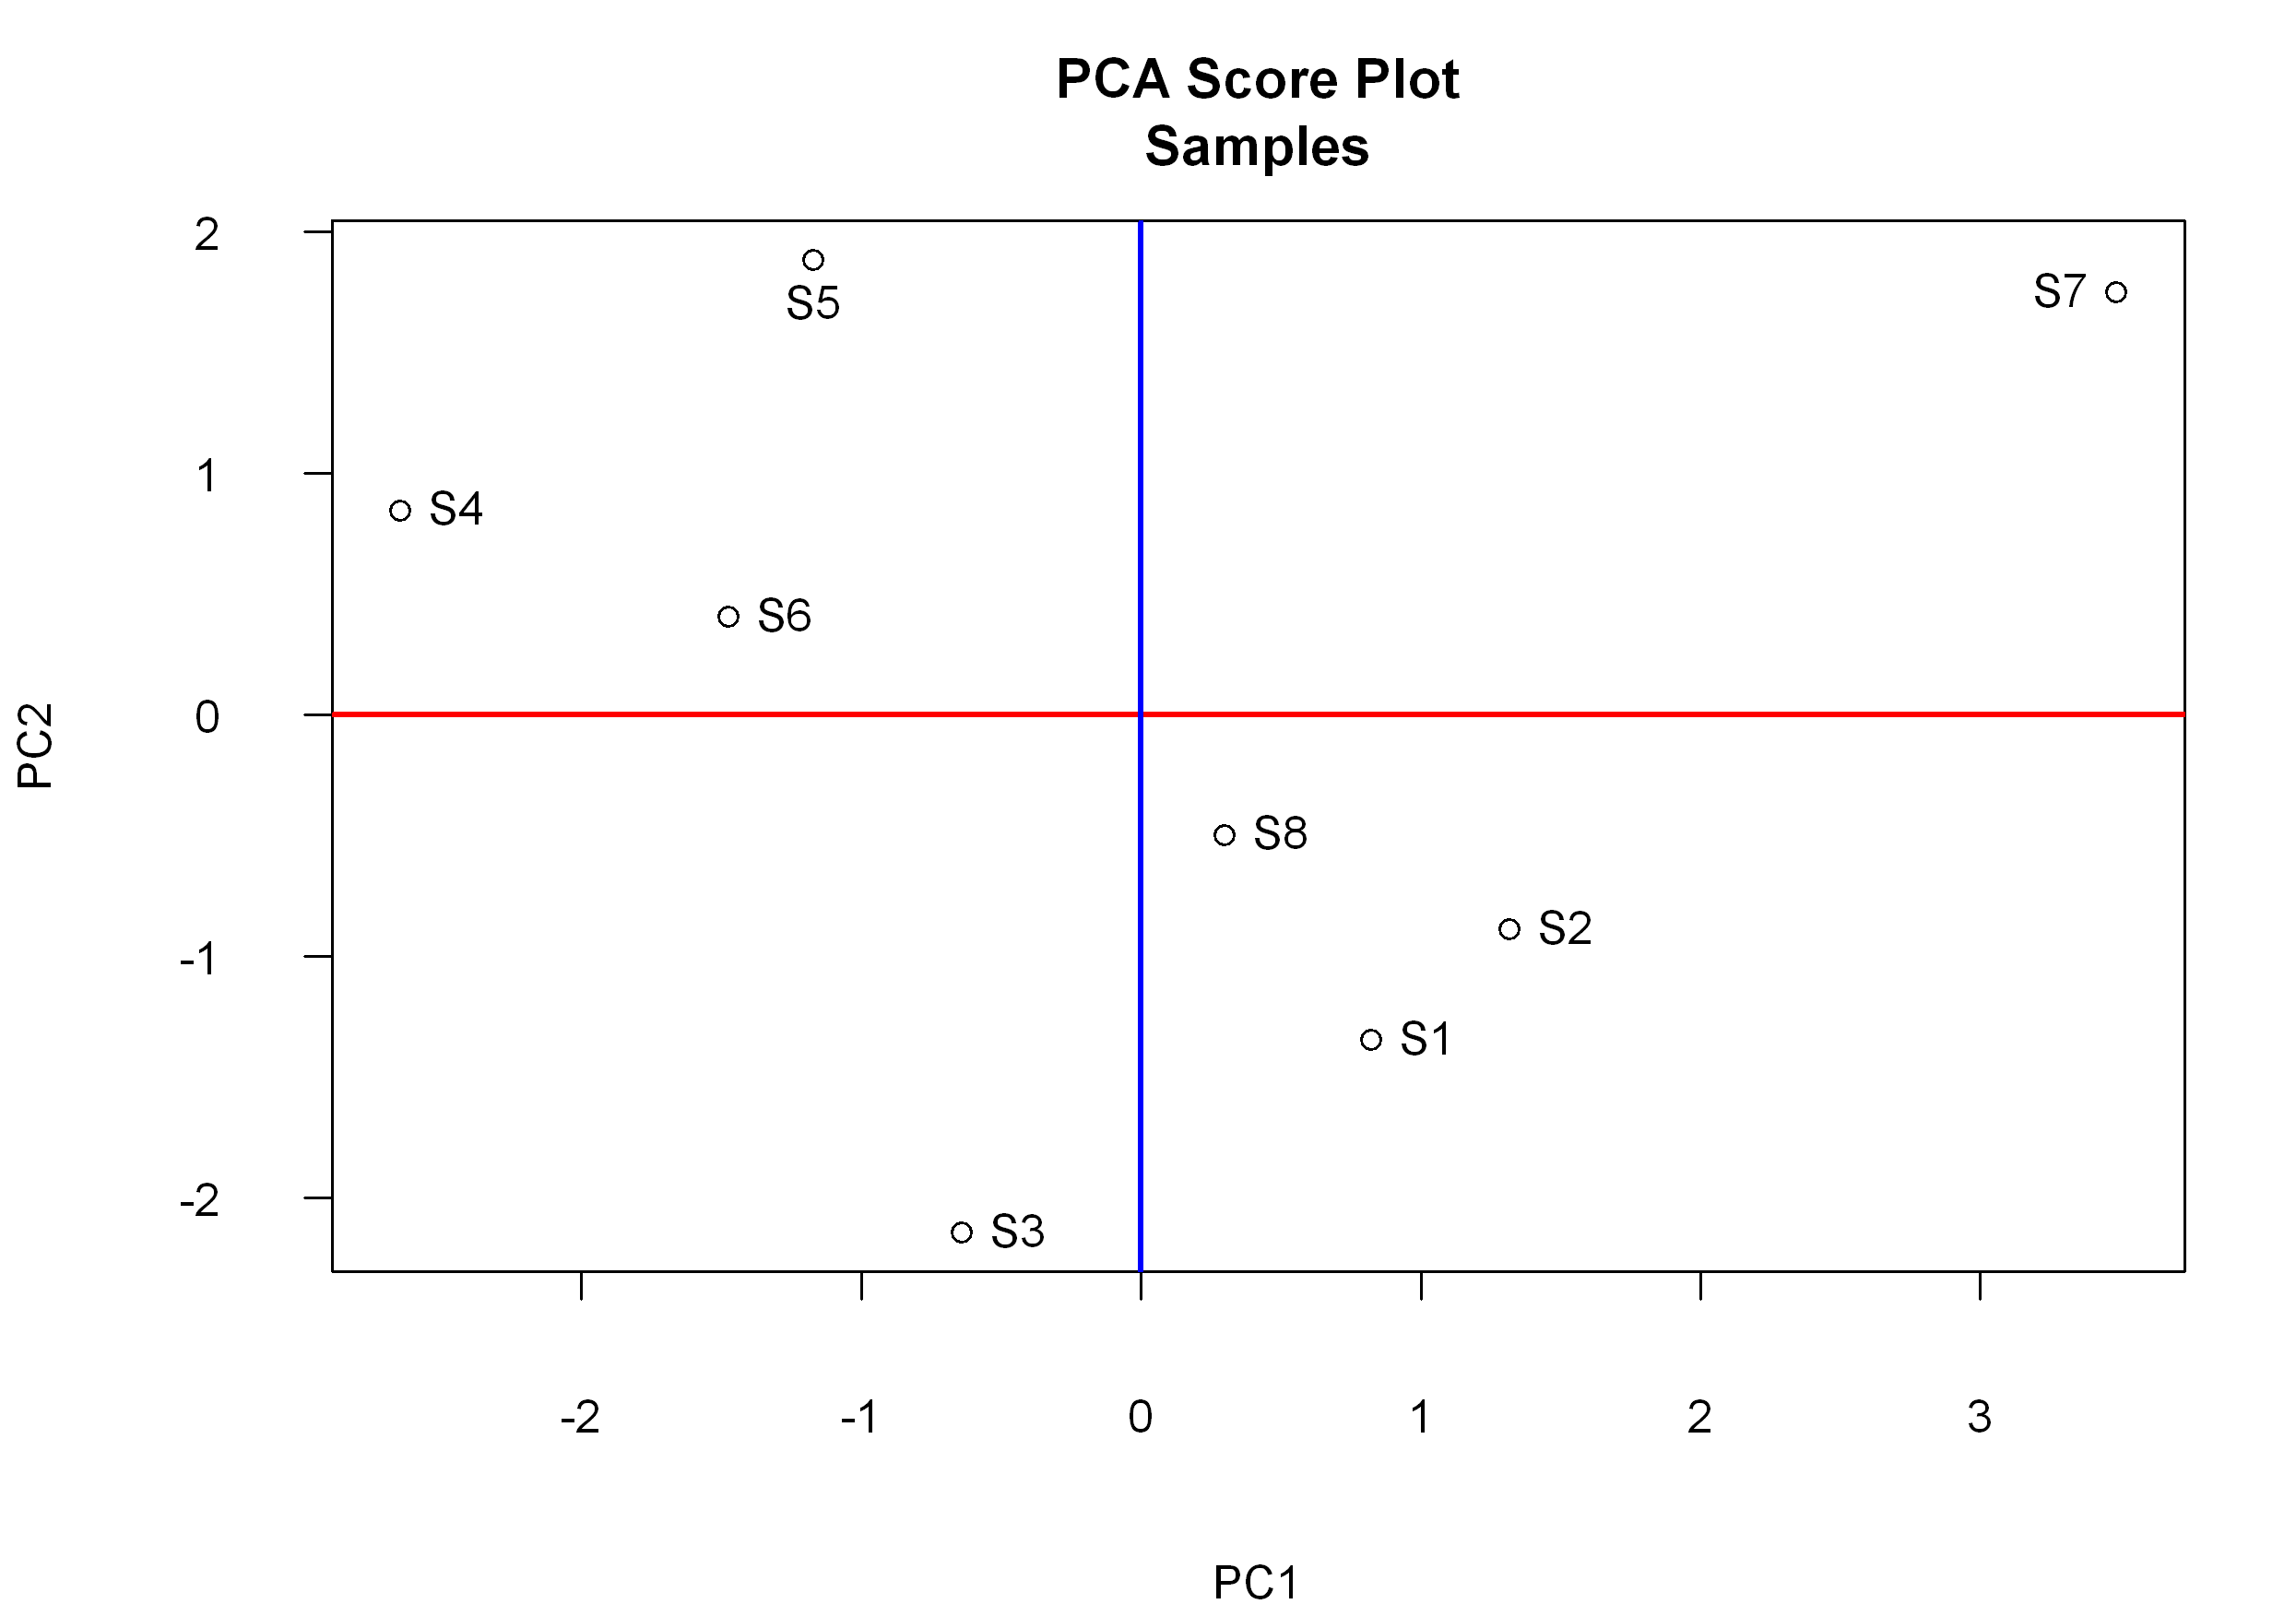
\includegraphics[width=0.85\textwidth]{images/PCA_scores_smpl.png} \\
    \caption[PCA - Scores (by sample)]{Scores plot with sample names as labels.}
    \label{fig:PCA_scores_smpl}
\end{figure}

\begin{figure}[!h!bp]
    \centering
    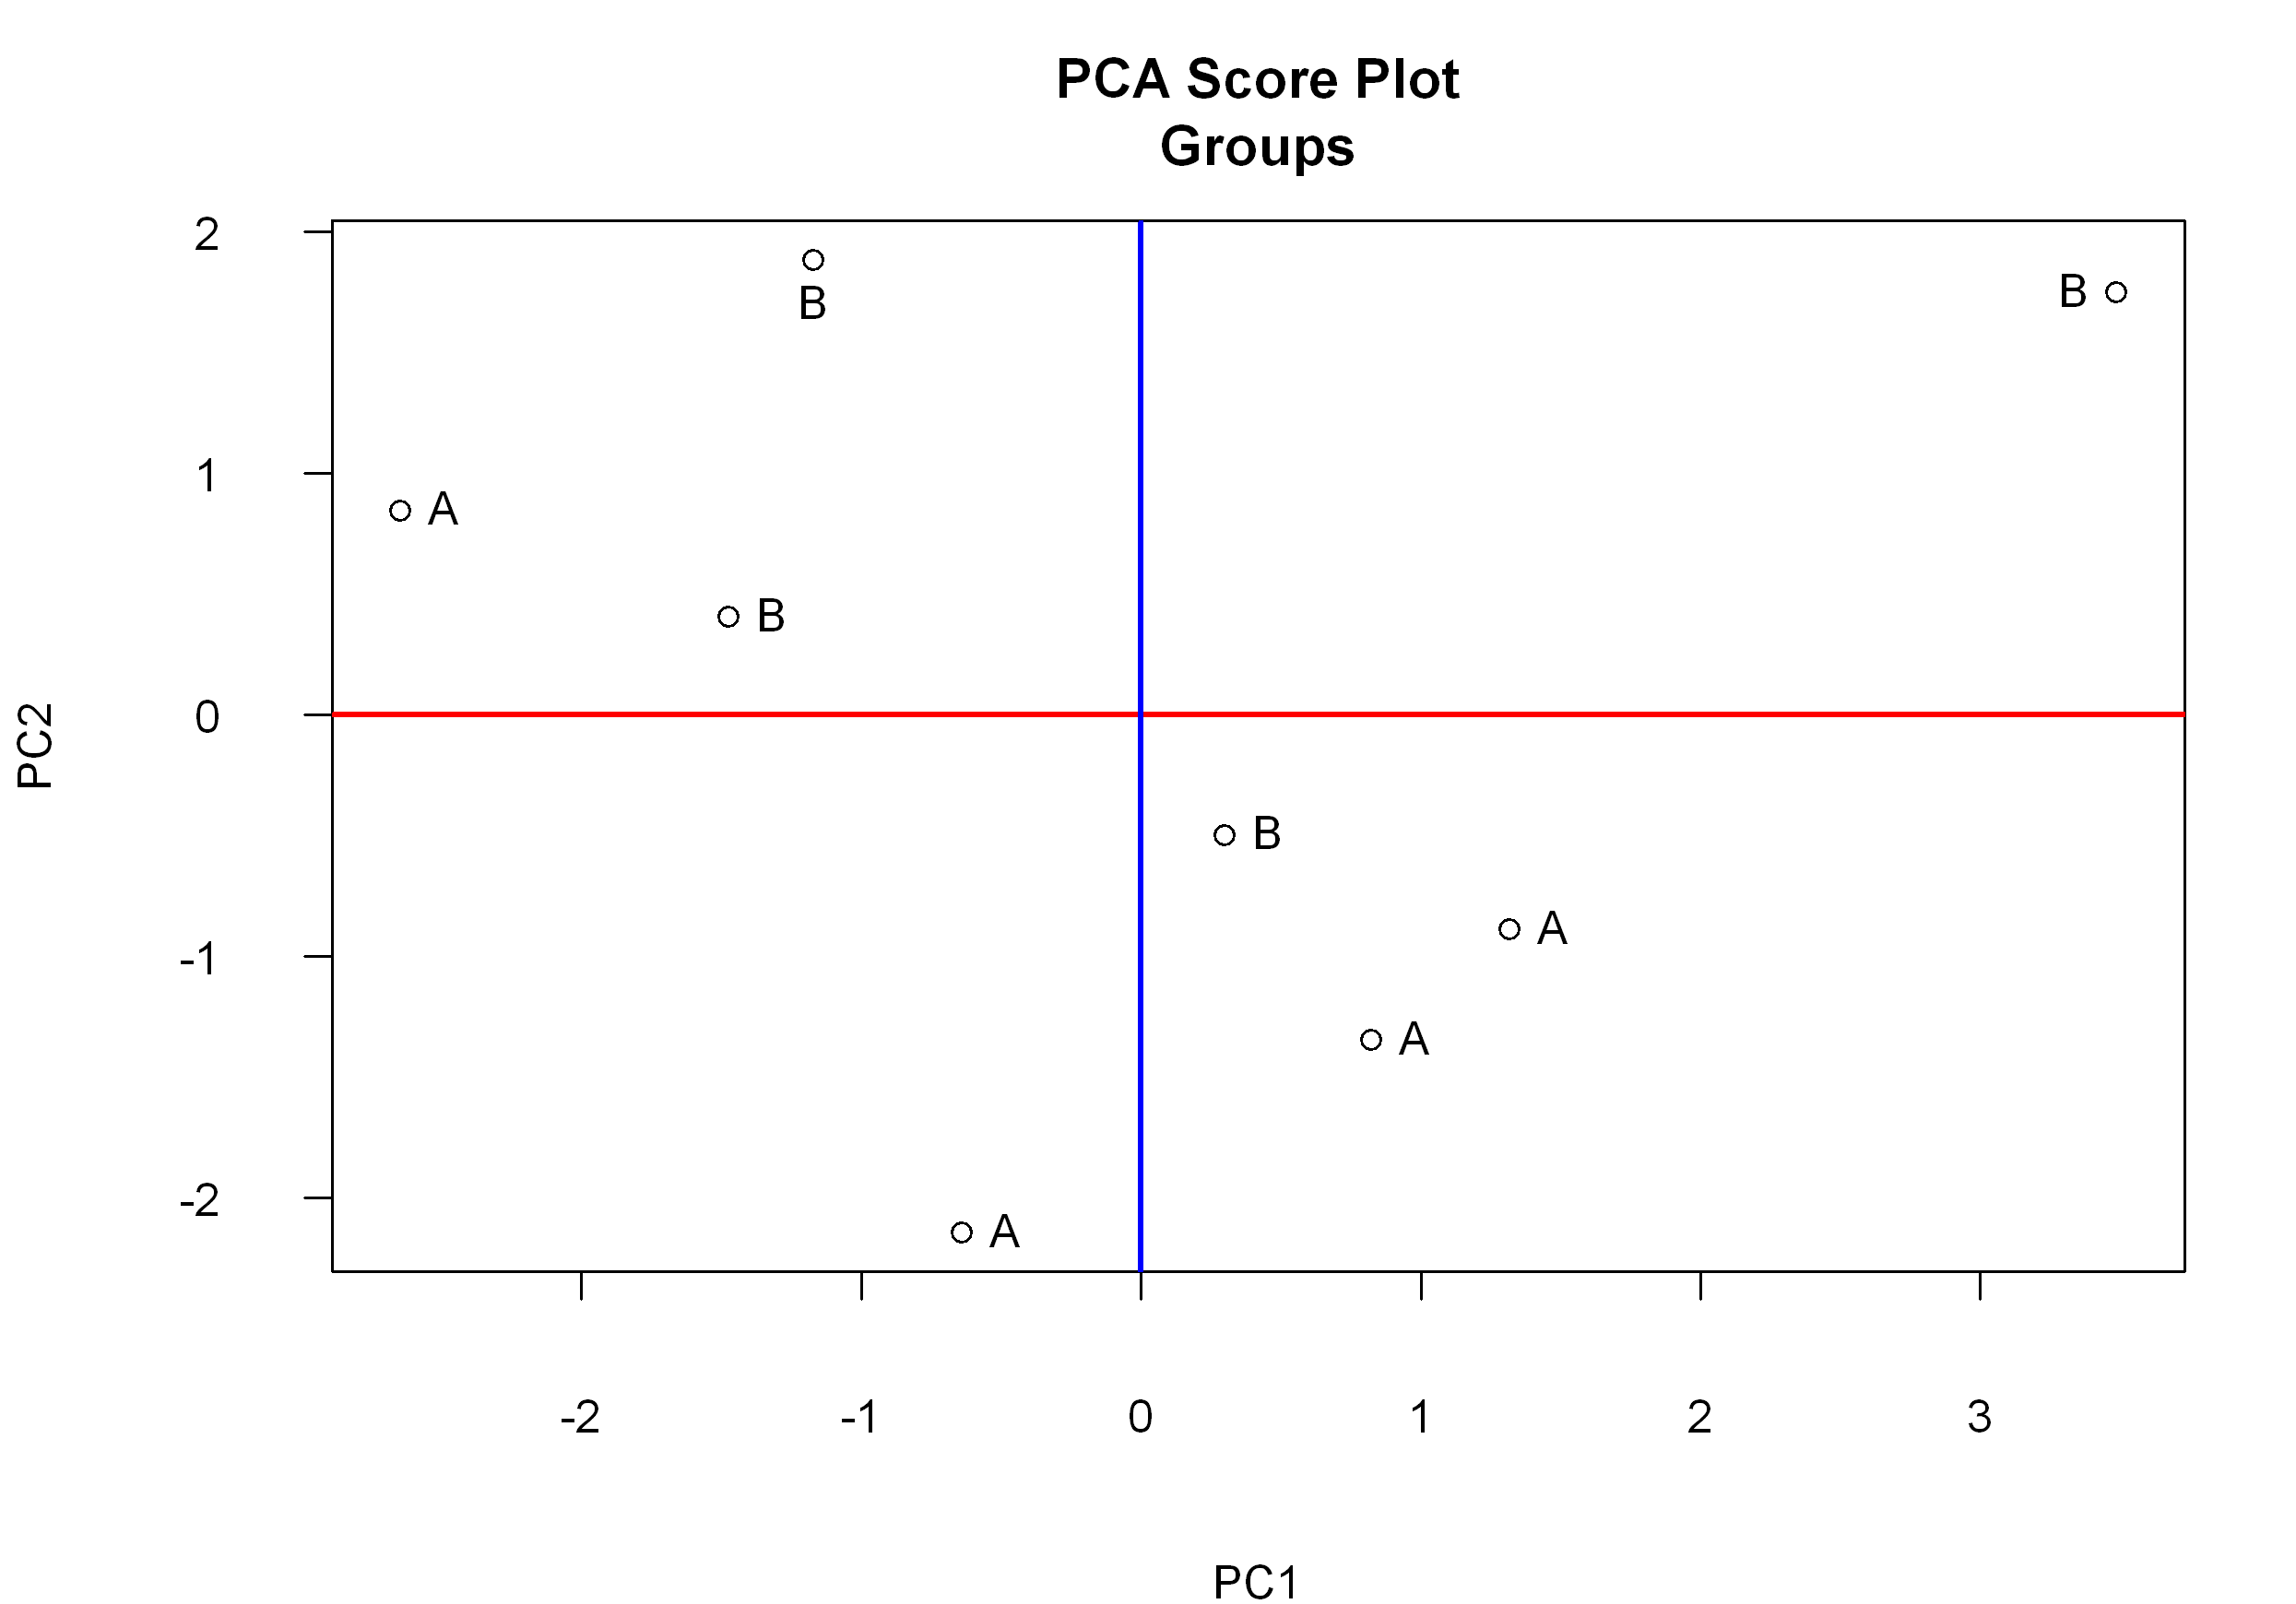
\includegraphics[width=0.85\textwidth]{images/PCA_scores_grp.png} \\
    \caption[PCA - Scores (by group)]{Scores plot with group names as labels.}
    \label{fig:PCA_scores_grp}
\end{figure}

\begin{figure}[!hp]
    \centering
    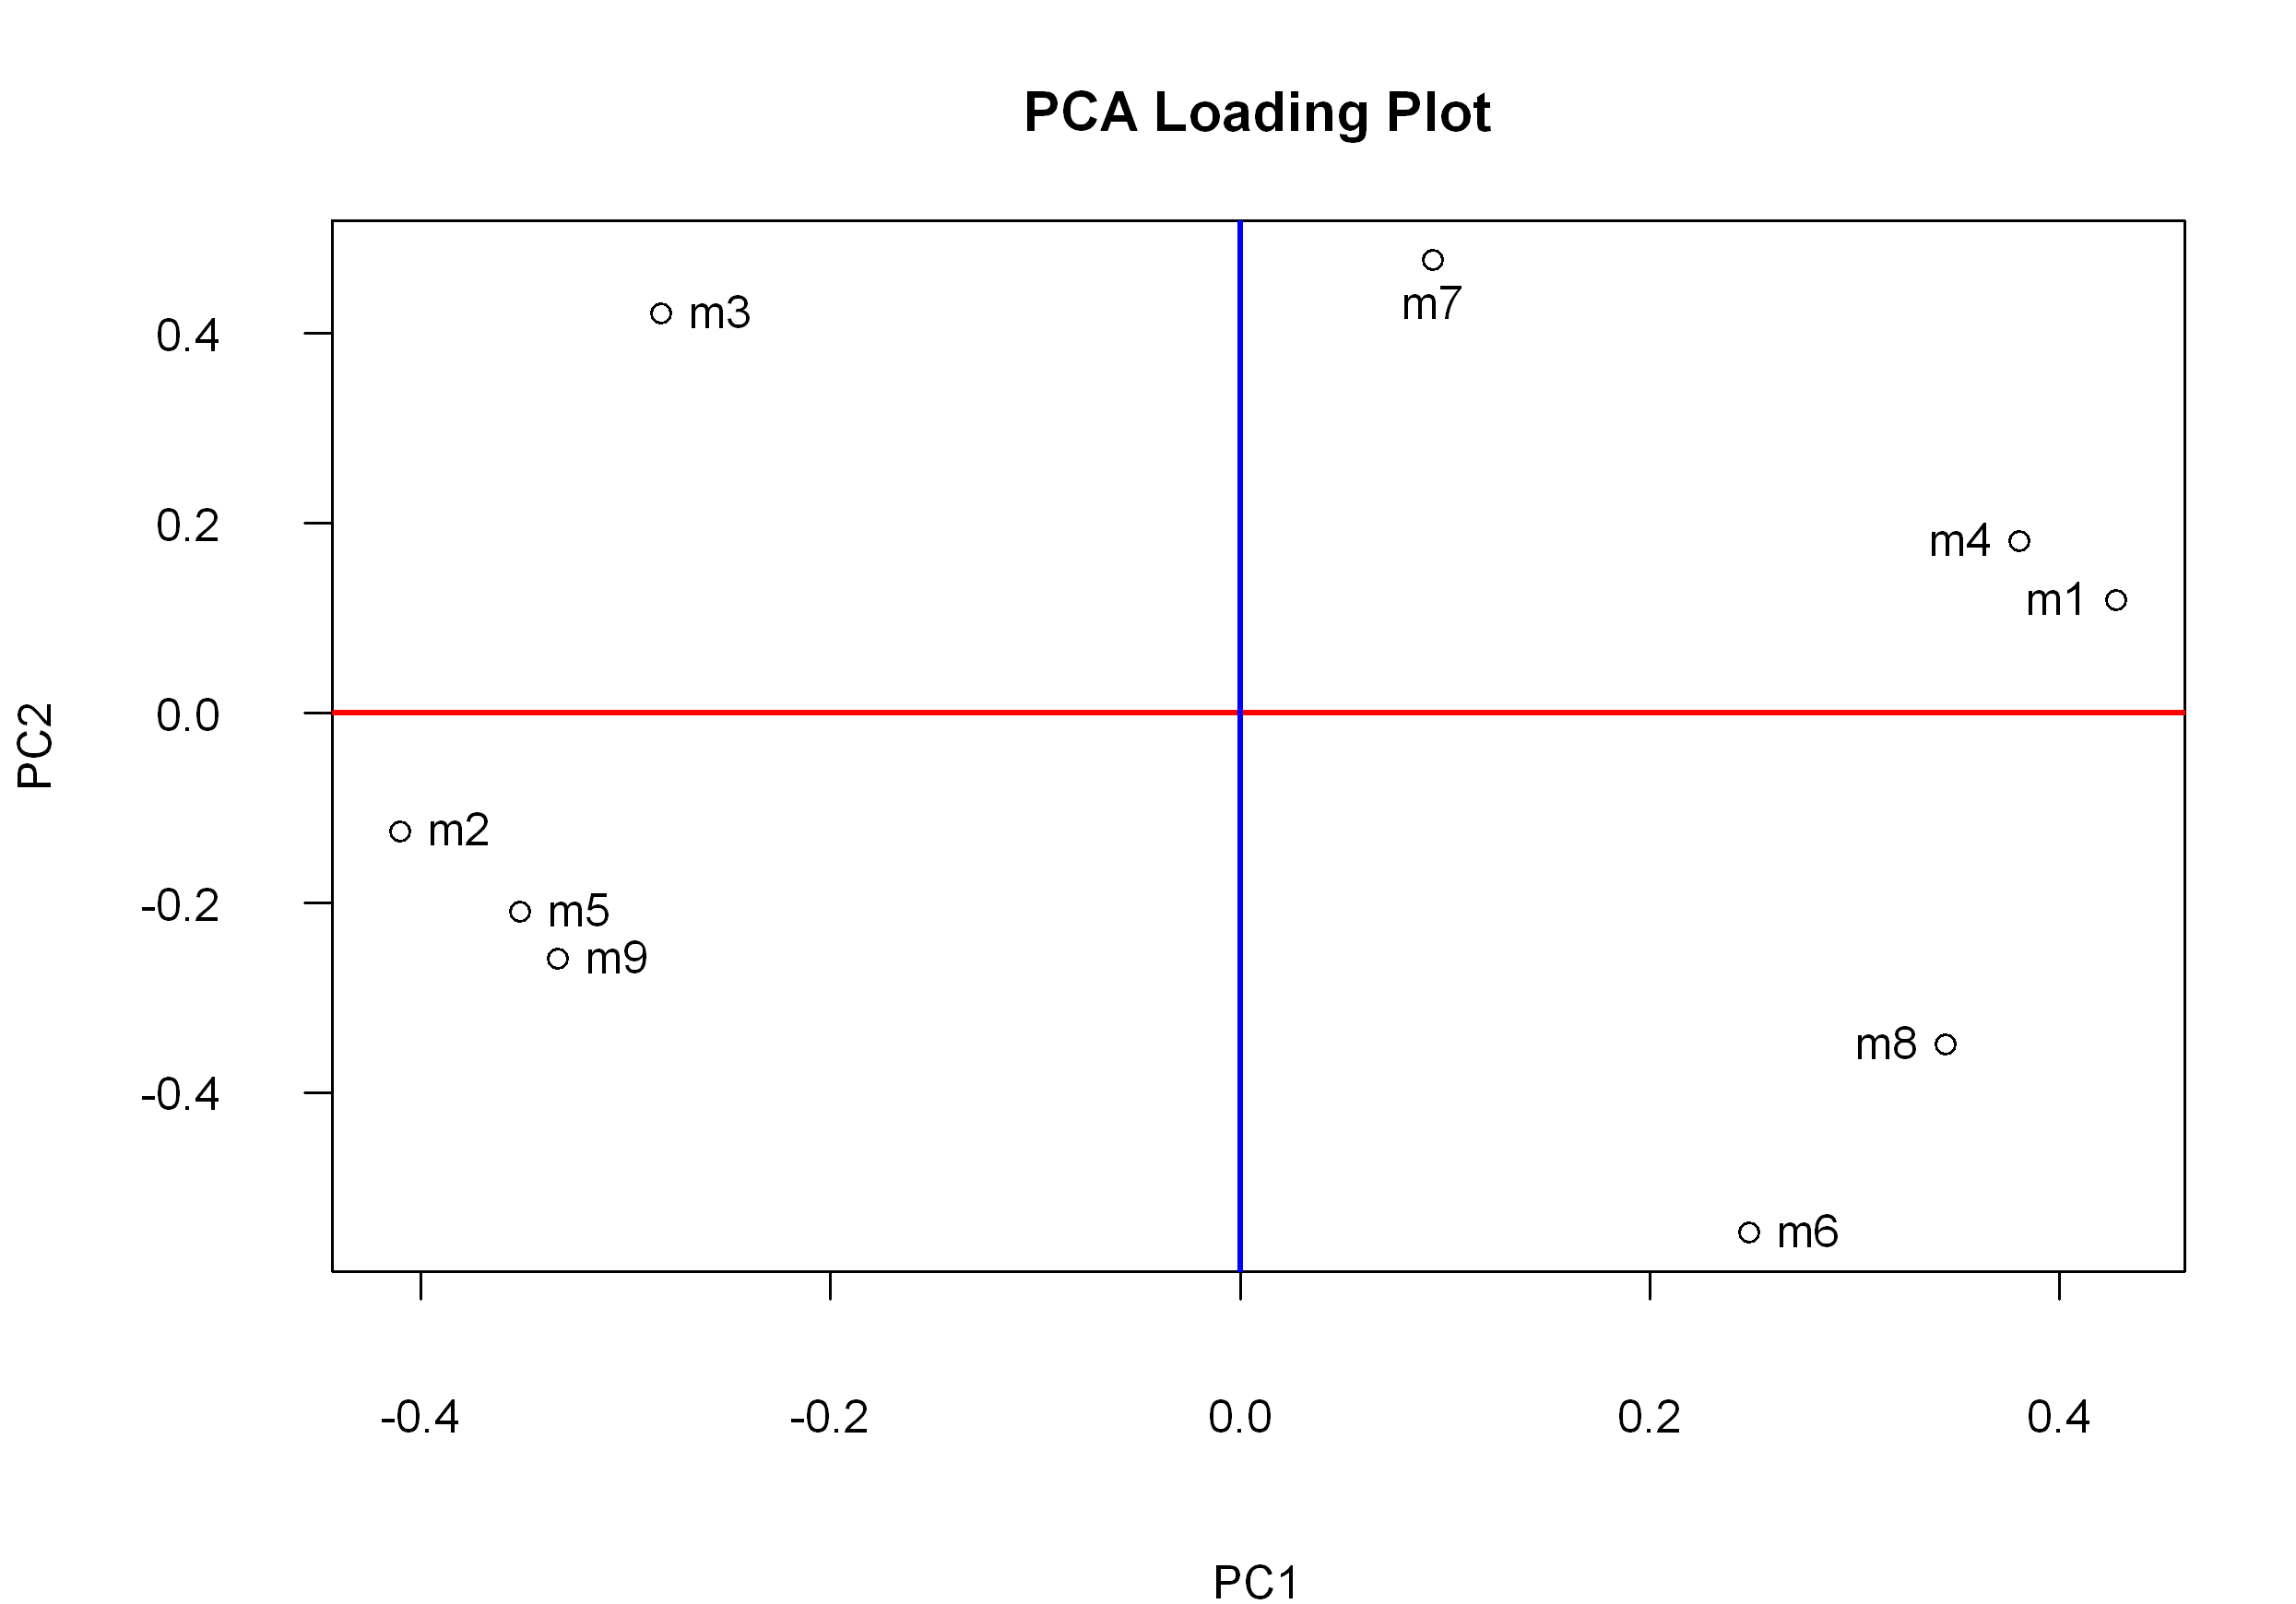
\includegraphics[width=0.85\textwidth]{images/PCA_loadings.png} \\
    \caption[PCA - Loadings]{Loadings plot. Indicates which variables contributed to the separation seen in the scores plot.}
    \label{fig:PCA_loadings}
\end{figure}

\subsubsection*{lda.r}
\addcontentsline{toc}{subsubsection}{lda.r}
Linear Discriminant Analysis (LDA) is a classical technique to predict groups of samples. This is a supervised method that requires prior knowledge of the groups. LDA is therefore well suited for non-targeted metabolic profiling data which is almost always ``grouped''. LDA is very similar to PCA, except that the technique maximises the ratio of between-class variance to the within-class variance in a set of data, and thus gives maximal separation between the classes, as shown in Figure \ref{fig:LDA}.

\begin{figure}[!h!tb]
    \centering
    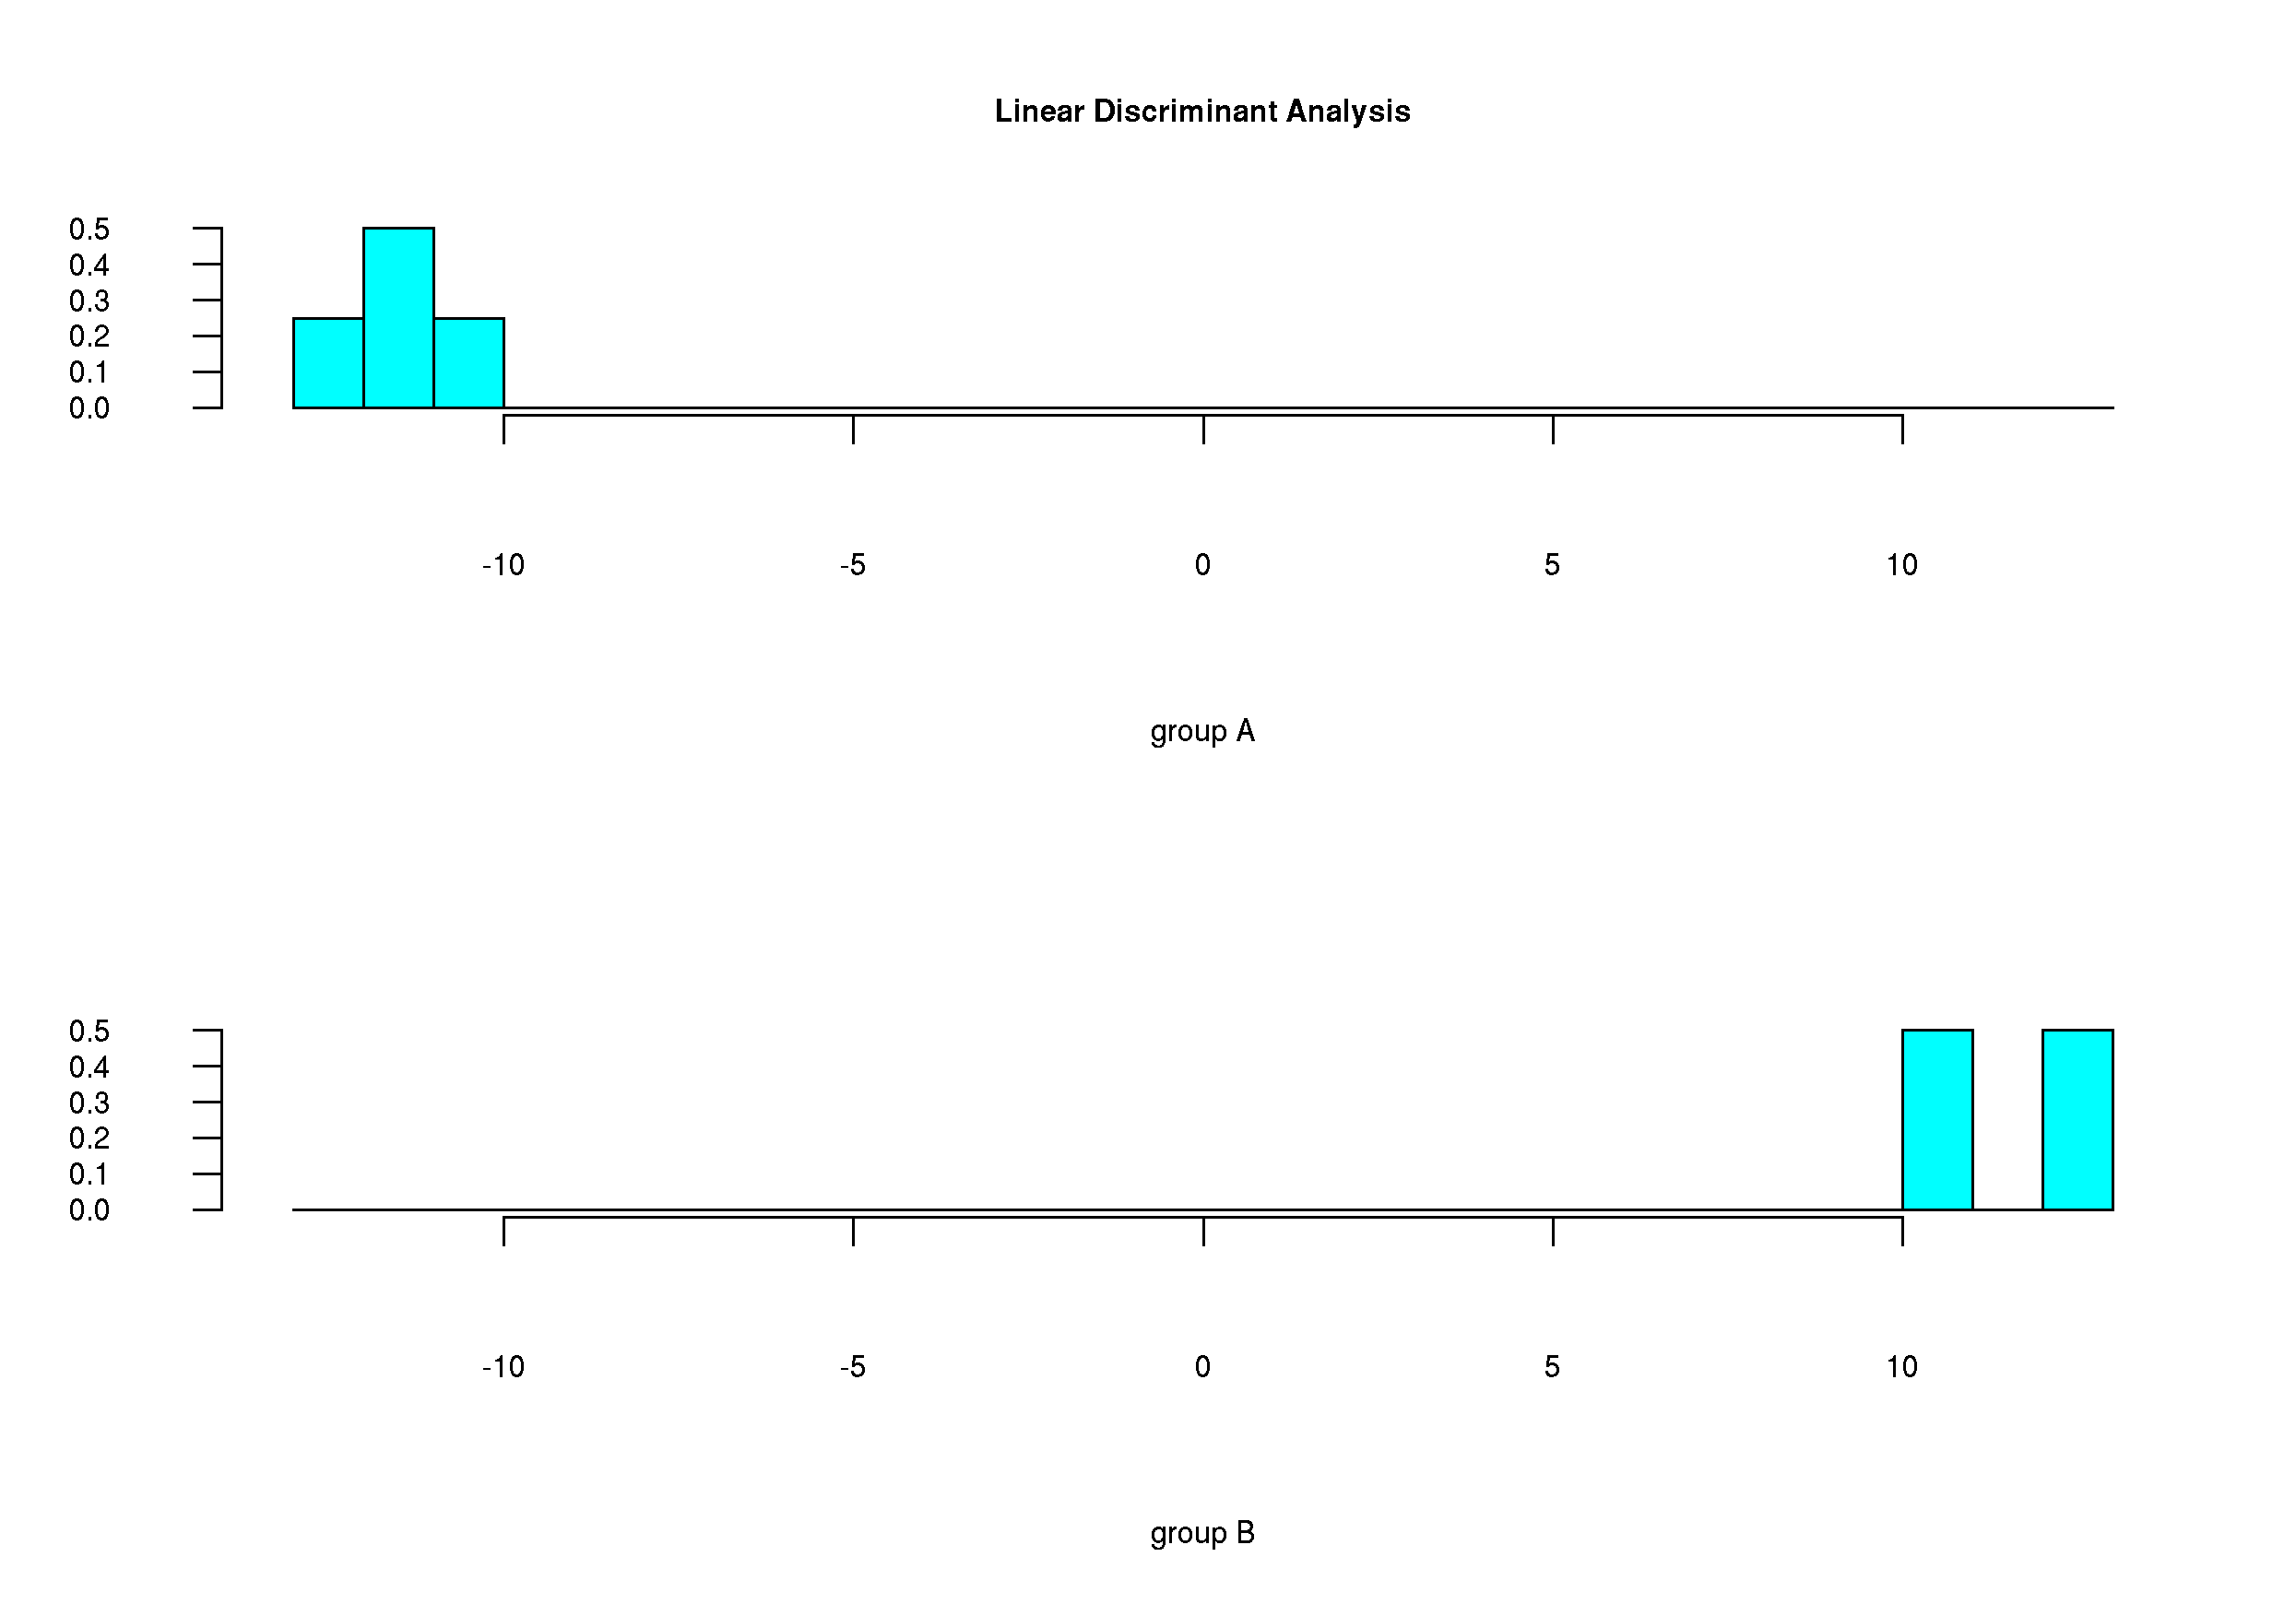
\includegraphics[width=0.85\textwidth]{images/LDA.png} \\
    \caption[Linear Discriminant Analysis]{Linear Discriminant Analysis for two groups. This example shows a very clear separation between the groups.}
    \label{fig:LDA}
\end{figure}

\subsubsection*{heatmap.r}
\addcontentsline{toc}{subsubsection}{heatmap.r}
Produces a hierarchical cluster dendogram for both samples (\emph{x}-axis) and variables (\emph{y}-axis), and uses colours to represent the values. This results in a readily interpretable figure as shown in Figure \ref{fig:heatmap}.

\begin{figure}[!h!bt]
    \centering
    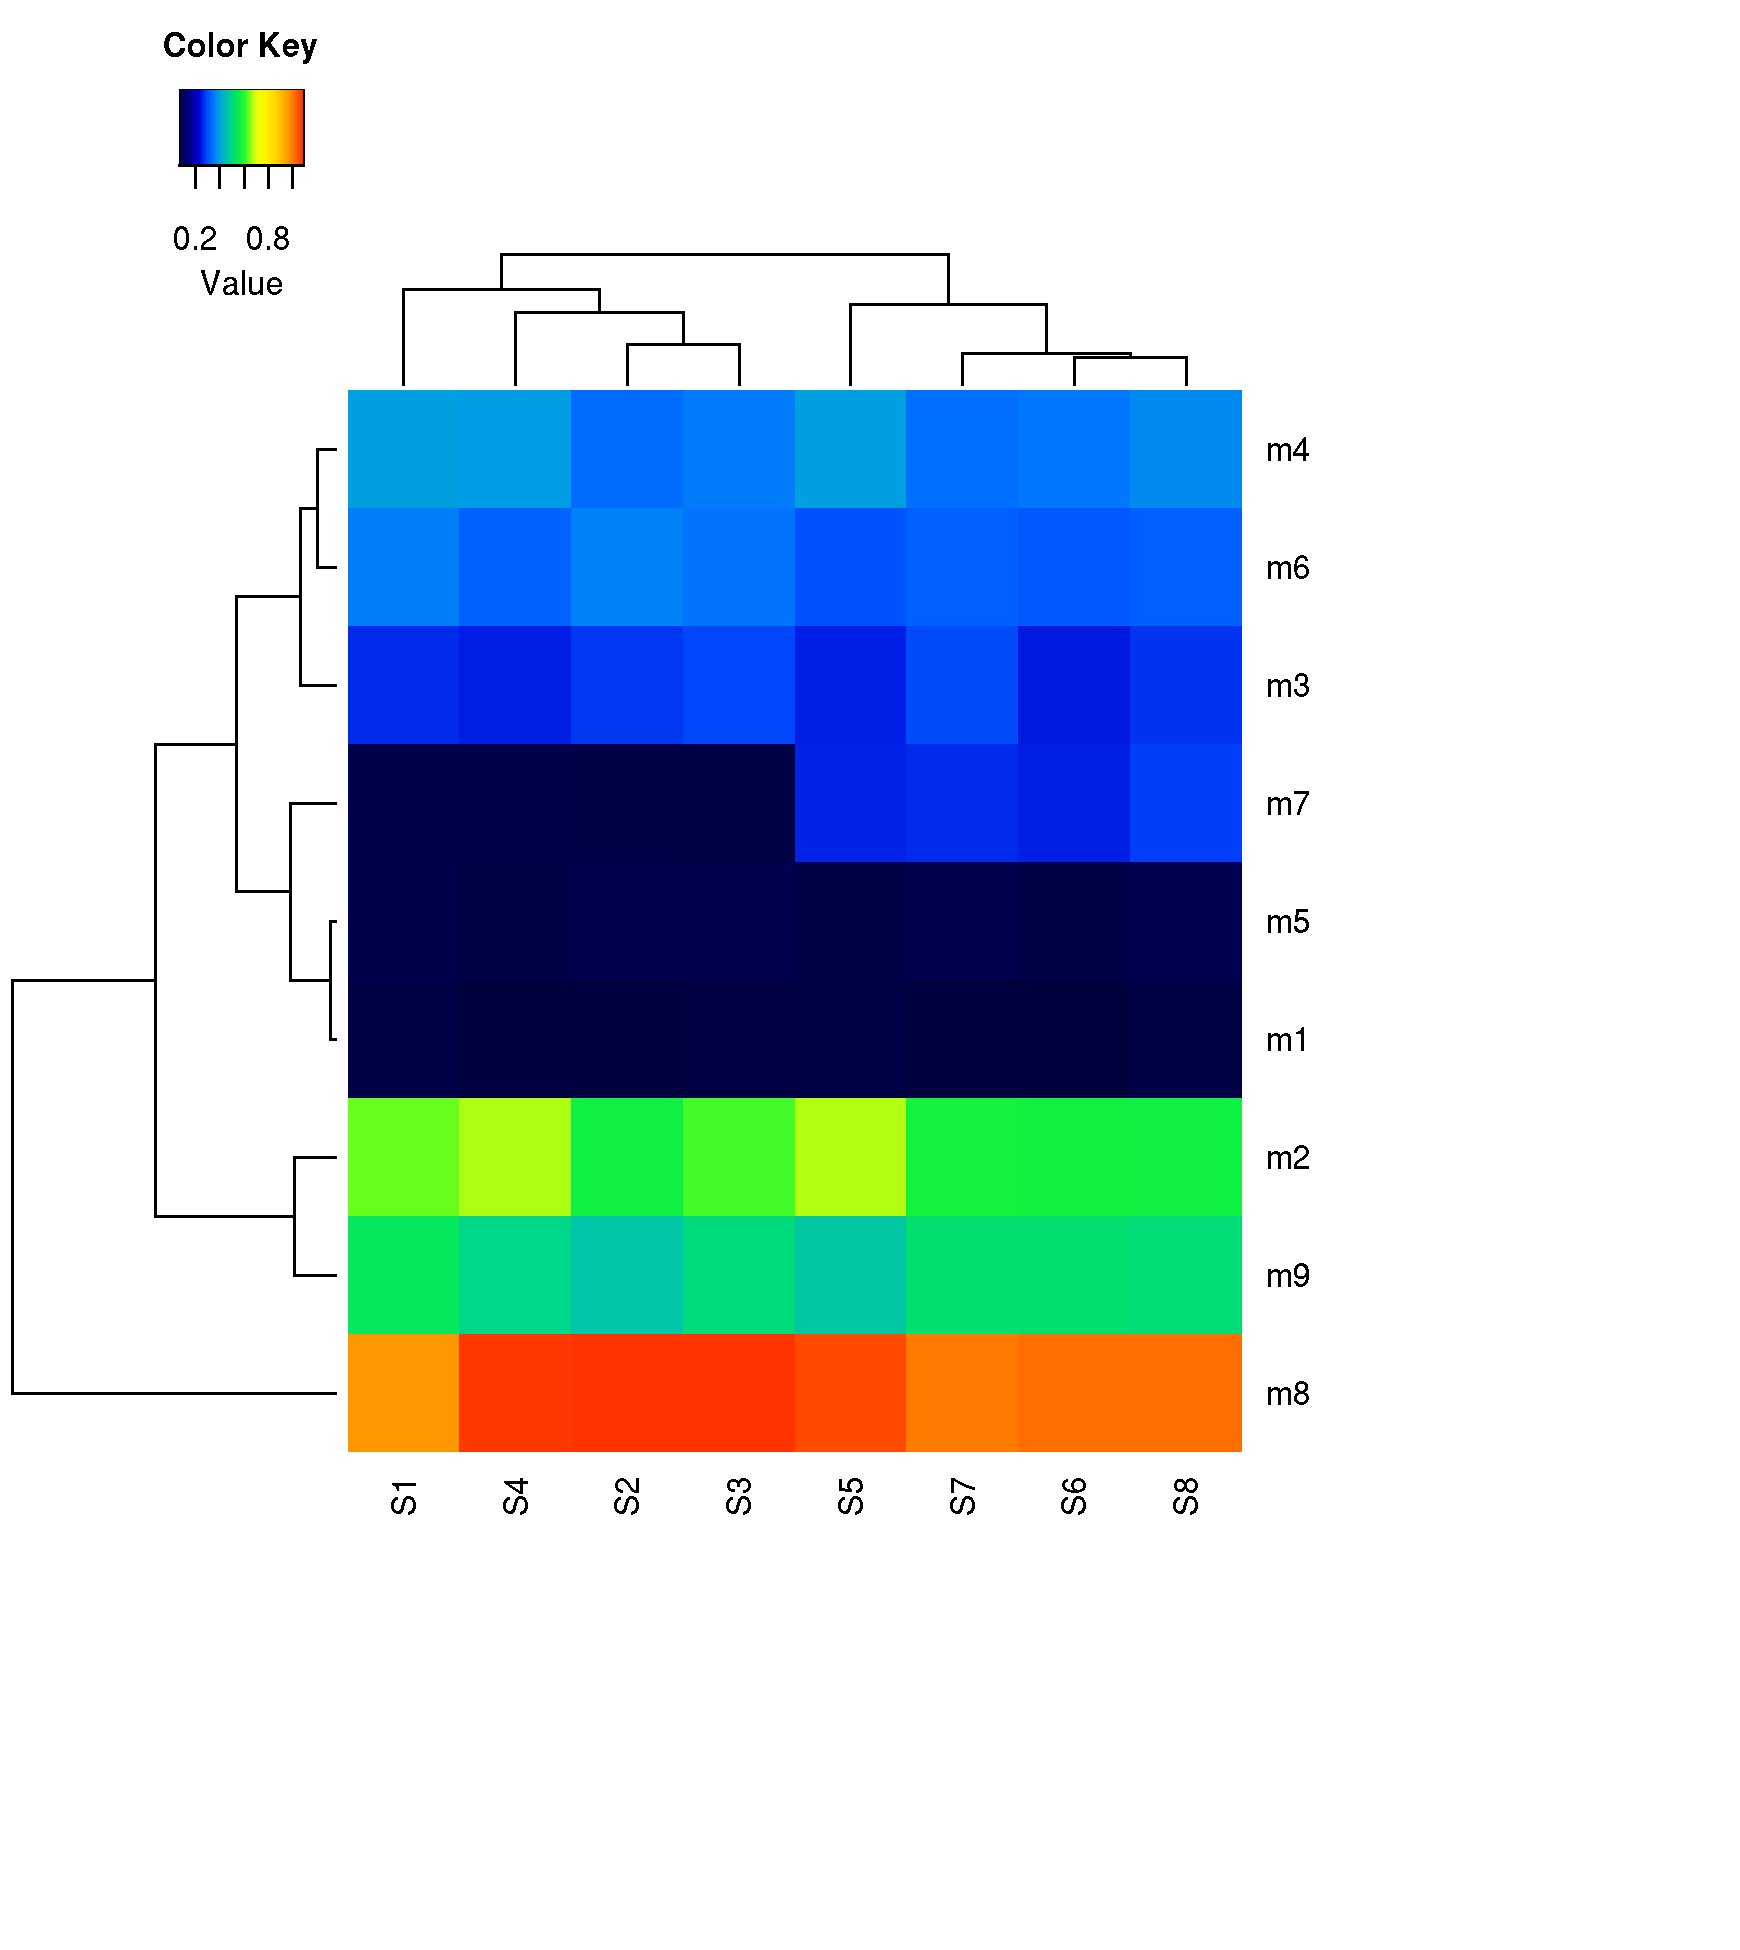
\includegraphics[width=0.85\textwidth]{images/heatmap.png} \\
    \caption[Heatmap]{Heatmap showing sample clustering along the \emph{x}-axis and metabolites along the \emph{y}-axis. The Color Key shows the value represented by the colours in the body of the plot.}
    \label{fig:heatmap}
\end{figure}

\end{document}
